%\VignetteEngine{knitr::knitr}
% some terminal commands to copy once and scroll when needed
% cd '/mnt/Hitachi2GB/00NMML/activePapers/spAReco/spAReco_package/spAReco/inst/doc'
% cd '/home/jay/Data/spAReco/spAReco_package/spAReco/inst/doc'
% Rscript -e "library(knitr); knit('spARecoEM.Rnw')"
% Rscript -e "library(knitr); purl('spARecoEM.Rnw')"
% pdflatex spARecoEM
% bibtex spARecoEM

\documentclass[11pt, titlepage]{article}\usepackage[]{graphicx}\usepackage[]{color}
%% maxwidth is the original width if it is less than linewidth
%% otherwise use linewidth (to make sure the graphics do not exceed the margin)
\makeatletter
\def\maxwidth{ %
  \ifdim\Gin@nat@width>\linewidth
    \linewidth
  \else
    \Gin@nat@width
  \fi
}
\makeatother

\definecolor{fgcolor}{rgb}{0.345, 0.345, 0.345}
\newcommand{\hlnum}[1]{\textcolor[rgb]{0.686,0.059,0.569}{#1}}%
\newcommand{\hlstr}[1]{\textcolor[rgb]{0.192,0.494,0.8}{#1}}%
\newcommand{\hlcom}[1]{\textcolor[rgb]{0.678,0.584,0.686}{\textit{#1}}}%
\newcommand{\hlopt}[1]{\textcolor[rgb]{0,0,0}{#1}}%
\newcommand{\hlstd}[1]{\textcolor[rgb]{0.345,0.345,0.345}{#1}}%
\newcommand{\hlkwa}[1]{\textcolor[rgb]{0.161,0.373,0.58}{\textbf{#1}}}%
\newcommand{\hlkwb}[1]{\textcolor[rgb]{0.69,0.353,0.396}{#1}}%
\newcommand{\hlkwc}[1]{\textcolor[rgb]{0.333,0.667,0.333}{#1}}%
\newcommand{\hlkwd}[1]{\textcolor[rgb]{0.737,0.353,0.396}{\textbf{#1}}}%

\usepackage{framed}
\makeatletter
\newenvironment{kframe}{%
 \def\at@end@of@kframe{}%
 \ifinner\ifhmode%
  \def\at@end@of@kframe{\end{minipage}}%
  \begin{minipage}{\columnwidth}%
 \fi\fi%
 \def\FrameCommand##1{\hskip\@totalleftmargin \hskip-\fboxsep
 \colorbox{shadecolor}{##1}\hskip-\fboxsep
     % There is no \\@totalrightmargin, so:
     \hskip-\linewidth \hskip-\@totalleftmargin \hskip\columnwidth}%
 \MakeFramed {\advance\hsize-\width
   \@totalleftmargin\z@ \linewidth\hsize
   \@setminipage}}%
 {\par\unskip\endMakeFramed%
 \at@end@of@kframe}
\makeatother

\definecolor{shadecolor}{rgb}{.97, .97, .97}
\definecolor{messagecolor}{rgb}{0, 0, 0}
\definecolor{warningcolor}{rgb}{1, 0, 1}
\definecolor{errorcolor}{rgb}{1, 0, 0}
\newenvironment{knitrout}{}{} % an empty environment to be redefined in TeX

\usepackage{alltt}
\usepackage{geometry}
\geometry{verbose,letterpaper,tmargin=2.54cm,bmargin=2.54cm,lmargin=2.54cm,rmargin=2.54cm}
\usepackage{graphicx, ams, amsmath, amssymb, natbib, setspace}
\usepackage{float}
\usepackage{multirow}
\usepackage{mathrsfs}
\usepackage{relsize}
\usepackage{subfigure}
\usepackage{pgf}
\usepackage{/mnt/Hitachi2GB/shTex/mymacros}
\usepackage{bbding}
\usepackage{lineno}
\usepackage{fancyvrb}
\usepackage[shortlabels]{enumitem}
\linenumbers
\setlength{\parindent}{3em} 
%\onehalfspacing
\doublespacing
\usepackage{lipsum}
\usepackage{setspace}
\usepackage{etoolbox}
\AtBeginEnvironment{tabular}{\singlespacing}
\pdfpagewidth 8.5in
\pdfpageheight 11in
\setlength{\oddsidemargin}{0.0in} \setlength{\textwidth}{6.5in}
\setlength{\topmargin}{0.15in} \setlength{\textheight}{8.5in}
\setlength{\headheight}{0.0in} \setlength{\headsep}{0.0in}
%\renewcommand{\abstractname}{Summary}
%\renewcommand{\theequation}{(\arabic{equation})}
\setcounter{figure}{0}
\makeatletter

%\renewcommand\tagform@[1]{\maketag@@@{\ignorespaces#1\unskip\@@italiccorr}}
\makeatother
\IfFileExists{upquote.sty}{\usepackage{upquote}}{}
\begin{document}


% ------------------------------------------------------------------------------
% ------------------------------------------------------------------------------
% 																	TITLE
% ------------------------------------------------------------------------------
% ------------------------------------------------------------------------------

\titlepage
\title {Spatial Autoregressive Models for Ecological Inference}
\author{Jay M. Ver Hoef$^1$, Erin E. Peterson$^2$, Mevin B. Hooten$^3$, Ephraim M. Hanks$^4$, and \\
	Marie-Jos\'{e}e Fortin$^5$ \\
\hrulefill \\ 
$^1$National Marine Mammal Laboratory, NOAA-NMFS Alaska Fisheries Science Center\\
7600 Sand Point Way NE, Seattle, WA 98115\\
tel: (907) 456-1995 \hspace{.5cm} E-mail: jay.verhoef@noaa.gov\\
$^2$ ARC Centre for Excellence in Mathematical and Statistical Frontiers (ACEMS) and \\
the Institute for Future Environments, Queensland University of Technology \\ 
$^3$ U.S. Geological Survey, Colorado Cooperative Fish and Wildlife Research Unit, \\
Department of Fish, Wildlife, and Conservation Biology \\
Department of Statistics, Colorado State University \\
$^4$ Department of Statistics, The Pennsylvania State University \\
$^5$ Department of Ecology and Evolutionary Biology, University of Toronto \\
\hrulefill \\
}

\maketitle

% ------------------------------------------------------------------------------
% ------------------------------------------------------------------------------
% ------------------------------------------------------------------------------
% 														   	ABSTRACT
% ------------------------------------------------------------------------------
% ------------------------------------------------------------------------------
% ------------------------------------------------------------------------------

\begin{abstract}
\begin{onehalfspace}

We review conditional autoregressive (CAR) and simultaneous autoregressive (SAR) models for spatial ecological data because they are under-used, or used incorrectly, and this is likely because they are more difficult to understand than geostatistical models. To highlight their usefulness, we identify and discuss six different types of ecological inference using CAR and SAR models, including model selection, spatial regression, estimation of autocorrelation, estimation of other connectivity parameters, spatial prediction, and spatial smoothing.  We compare and contrast CAR and SAR models, showing their development and connection to partial correlations.  Special cases, such as the intrinsic autoregressive model (IAR), are also shown.  Practical use of CAR and SAR models depends on weight matrices, and neighborhood definition and row-standardization are important concepts when developing such matrices. Weight matrices can also include ecological covariates and connectivity structures, which we emphasize but have been rarely used. Trends in harbor seals (\emph{Phoca vitulina}) in southeastern Alaska from 463 polygons, some with missing data, are used to illustrate the six inference types and highlight discussion points from the earlier review. We develop a variety of weight matrices and corresponding CAR and SAR models are fit to data using maximum likelihood and Bayesian methods. We compare models and present spatial regression results for several of these models. Profile likelihood graphs illustrate inference for covariance parameters. The same data set is used for both prediction and smoothing, and the relative merits of each are discussed.  We show the nonstationary variances and correlations of a CAR model and demonstrate the effect of row-standardization. We highlight several reasons why ecologists will want to make use of autoregressive models, both directly and in hierarchical models, and not only in explicit spatial settings, but also for more general connectivity models (also known graphical models in mathematics). We conclude with some take-home messages for CAR and SAR models, including 1) thoughts on choosing between CAR and IAR models, 2) modeling ecological effects in the covariance matrix, 3) the appeal of spatial smoothing, 4) how to handle isolated neighbors, and 5) software considerations.
\end{onehalfspace}
\hrulefill \\

\noindent {\sc Key Words:} Conditional autoregressive, simultaneous autoregressive, CAR, SAR, IAR, geostatistics, prediction, smoothing\\

\end{abstract}

% ------------------------------------------------------------------------------
% ------------------------------------------------------------------------------
% ------------------------------------------------------------------------------
% 															INTRODUCTION
% ------------------------------------------------------------------------------
% ------------------------------------------------------------------------------
% ------------------------------------------------------------------------------

\newpage
\begin{spacing}{1.9}
\begin{flushleft}
\setlength{\parindent}{1cm}



\section*{INTRODUCTION}

Ecologists almost always collect spatial data, and these data often exhibit autocorrelation.  Autocorrelation is the tendency for sites that are close together to have more similar values than sites that are farther from each other.  In a spatial statistical model, this tendency of sites to covary, more at shorter distances and less at greater distances, is captured in the covariance matrix.  While it is a useful heuristic to describe such models based on distances between sites, not all spatial statistical models use distance directly. When data are collected at spatial locations, \citet[][p. 8]{Cres:stat:1993} divides spatial statistical models into two broad classes: 1) point-referenced geostatistical models, and 2) lattice models, also called areal models \citep{Bane:Carl:Gelf:hier:2014}.  While the covariance matrix in a geostatistical model depends on distances among sites, consider the following simple example of 9 sites in a 3 $\times$ 3 grid,
\[
	\begin{array}{ccc}
		1 & 2 & 3 \\
		4 & 5 & 6 \\
		7 & 8 & 9 \\
	\end{array}
\]
where the numbers label each site.  Note that we do not give a coordinate system.  Rather than defining spatial relationships by distance, the lattice models define it by neighbors.  In this example, suppose that neigbhors are defined by the adjoining site, either vertically or horizontally, so site 1 has two neighbors, labeled 2 and 4, etc.  Like a covariance matrix, we can capture neighborhood relationships in a matrix.  For this example, let

\[
\renewcommand\arraystretch{.5}
\bW = \left(
\begin{array}{ccccccccc}
% latex table generated in R 3.2.4 by xtable 1.7-4 package
% Wed Jun  8 18:02:53 2016
 0 & 1 & 0 & 1 & 0 & 0 & 0 & 0 & 0 \\ 
  1 & 0 & 1 & 0 & 1 & 0 & 0 & 0 & 0 \\ 
  0 & 1 & 0 & 0 & 0 & 1 & 0 & 0 & 0 \\ 
  1 & 0 & 0 & 0 & 1 & 0 & 1 & 0 & 0 \\ 
  0 & 1 & 0 & 1 & 0 & 1 & 0 & 1 & 0 \\ 
  0 & 0 & 1 & 0 & 1 & 0 & 0 & 0 & 1 \\ 
  0 & 0 & 0 & 1 & 0 & 0 & 0 & 1 & 0 \\ 
  0 & 0 & 0 & 0 & 1 & 0 & 1 & 0 & 1 \\ 
  0 & 0 & 0 & 0 & 0 & 1 & 0 & 1 & 0 \\ 
  
\end{array}
\right)
\]
be a matrix that indicates neighbor relationships, where the $j$th column for the $i$th row indicates whether site $j$ is a neighbor of site $i$.  Now, the neighborhood matrix $\bW$ can be turned into a covariance matrix by using 
{
\[
\renewcommand\arraystretch{.5}
\bSigma = (\bI - \rho\bW)\upi  = \left(
\begin{array}{ccccccccc}
% latex table generated in R 3.2.4 by xtable 1.7-4 package
% Wed Jun  8 18:02:53 2016
 1.10 & 0.26 & 0.06 & 0.26 & 0.12 & 0.04 & 0.06 & 0.04 & 0.02 \\ 
  0.26 & 1.16 & 0.26 & 0.12 & 0.29 & 0.12 & 0.04 & 0.07 & 0.04 \\ 
  0.06 & 0.26 & 1.10 & 0.04 & 0.12 & 0.26 & 0.02 & 0.04 & 0.06 \\ 
  0.26 & 0.12 & 0.04 & 1.16 & 0.29 & 0.07 & 0.26 & 0.12 & 0.04 \\ 
  0.12 & 0.29 & 0.12 & 0.29 & 1.24 & 0.29 & 0.12 & 0.29 & 0.12 \\ 
  0.04 & 0.12 & 0.26 & 0.07 & 0.29 & 1.16 & 0.04 & 0.12 & 0.26 \\ 
  0.06 & 0.04 & 0.02 & 0.26 & 0.12 & 0.04 & 1.10 & 0.26 & 0.06 \\ 
  0.04 & 0.07 & 0.04 & 0.12 & 0.29 & 0.12 & 0.26 & 1.16 & 0.26 \\ 
  0.02 & 0.04 & 0.06 & 0.04 & 0.12 & 0.26 & 0.06 & 0.26 & 1.10 \\ 
  
\end{array}
\right)
\]
}
where $\bI$ is a diagonal matrix of all 1's and $\rho=0.2$.  Notice that for the covariance matrix $\bSigma$, site 1 is most highly correlated with sites 2 and 4, based on the neighborhood definition.  We use this simple example to make two important distinctions between geostatistical models and lattice models: 1) geostatistical models are defined by actual spatial distance, while lattice models are defined by neighborhoods, and 2) geostatistics models specify the covariance matrix directly, whereas lattice models specify, essentially, the inverse of the covariance matrix when using neighborhoods.

When data are collected at spatial locations, \citet[][p. 8]{Cres:stat:1993} divides spatial statistical models into two broad classes: 1) point-referenced geostatistical models, and 2) lattice models, also called areal models \citep{Bane:Carl:Gelf:hier:2014}.  The two most common lattice models are the conditional autoregressive (CAR) and simultaneous autoregressive (SAR) models. The defining characteristic for CAR and SAR models is that the data occur on a (possibly irregular) grid, or lattice, with a countable set of nodes.  Geostatistical models, on the other hand, are used for data that are spatially continuous (i.e., a continuous surface). Another distinction that we find more useful for conceptual understanding is that geostatical models use spatial information to directly model a covariance matrix, whereas CAR and SAR models use spatial information to model the inverse of a covariance matrix (also known as the precision matrix).  Modeling the precision matrix is less intuitive than modeling the covariance matrix, which may make it more difficult to understand the implications of modeling decisions.  Indeed, in certain circumstances, \citet{Wall:clos:2004} found some surprising and unusual behavior for CAR and SAR models. The less intuitive precision matrix, and a reputation for unusual behavior, may unfortunately keep some scientists from using these models, or inference from the model may be used incorrectly. For example, some highly cited ecological papers have incorrectly compared CAR/SAR to geostatistical models, incorrectly formulated the CAR model, and have given incorrect relationships between CAR and SAR models. We do not dwell on these (details are given in Appendix A), but rather they illustrate that good statistical practice with CAR and SAR models depends on more and better information. CAR and SAR models have many useful applications \citep[e.g.,][]{Gelf:Schm:Wu:Sila:Lati:mode:2005, Lati:Wu:Gelf:Sila:buil:2006, Mago:Ray:John:Valk:Daws:Bowm:mode:2007, Hank:Hoot:circ:2013}.  Our objective is to review CAR and SAR models in a practical way, so that their potential may be more fully realized and used by ecologists.

First we motivate the uses of spatial autoregressive models with typical (and not so typical, but useful) objectives for ecological studies (Table~\ref{Tab:ARobj}). For objective 1, model selection, there are a plethora of model comparison methods, or multimodel inferences, based on Akaike Information Criteria \citep[AIC,][]{Akai:Info:1973}, Bayes Information Criteria \citep[BIC,][]{Schw:esti:1978}, etc., that are generally available \citep[see, e.g.,][]{Burn:Ande:mode:2002,Hoot:Hobb:guid:2015}.  CAR and SAR covariance matrices may be part of some or all models, and choosing a model, or comparing various CAR and SAR models, may be an important goal of the investigation. In recent theoretical developments, \citet{Song:DeOl:Baye:2012} provided details on comparing various CAR and SAR models by using Bayes factors. \citet{Zhu:Huan:Reye:sele:2010} extended the least absolute shrinkage and selection operator \citep[LASSO, ][]{Tibs:regr:1996} using the least angle regression algorithm \citep[LARS, ][]{Efro:Hast:John:Tibs:leas:2004} to CAR and SAR models. For applied examples, \citet{Cass:Dini:Rang:Thia:spat:2007} compared classical regression models assuming independence with SAR models while simultaneously selecting covariates using AIC while studying metabolism in amphibians. \citet{Qui:Turn:impo:2015} used SAR models for random errors along with model averaging in a study of landscape heterogeneity. \citet{Togn:Kelt:anal:2004} compared CAR and SAR based on autocorrelation in residuals, choosing SAR for an analysis of factors affecting mammalian species richness in South America.

For objective 2, regression, an early and influential paper on using CAR models for Scottish lip cancer data \citep{Clay:Kald:empi:1987} found that the covariate ``\% agriculture'' helped explain lip cancer rates among counties in Scotland, in conjunction with a CAR model for spatial autocorrelation in the errors.  For another example, a spatial CAR regression model using wolverine data \citep{Gard:Lawl:Ver:Mago:Kell:coar:2010} showed the probability of occupancy depended on covariates related to elevation and human influence in the plots. Returning to an example above, \citet{Cass:Dini:Rang:Thia:spat:2007} found that several environmental predictors, including temperature, net primary productivity, annual actual precipitation, etc., helped explain species richness of amphibians.  \citet{Agar:Sila:Gelf:Dewa:Mick:trop:2005} used a CAR error model to study the effect of landscape variables, including road and population density, on deforestation.  Using a SAR model for invasive alien plant species, \citet{Dark:biog:2004} found relationships with elevation, road density, and native plant species richness. In many of these models, the autoregressive component was a latent random effect in a generalized linear mixed model, or a hierarchical model, where the response variable was counts \citep{Clay:Kald:empi:1987}, binary \citep{Gard:Lawl:Ver:Mago:Kell:coar:2010}, or ordinal \citep{Agar:Sila:Gelf:Dewa:Mick:trop:2005}.  Later, we provide more discussion of CAR and SAR in hierarchical models.

\citet{Gard:Lawl:Ver:Mago:Kell:coar:2010} provided an example for objective 3, autocorrelation, using a Bayesian CAR model to estimate the autocorrelation parameter, along with credible intervals. \citet{Lich:Simo:Shri:Fran:spat:2002} also provided estimates of the CAR autocorrelation parameter for three different bird species, along with likelihood ratio tests against the null hypothesis that they were zero.  Similarly, but for SAR models, \citet{Bull:Burk:eval:2005} used likelihood ratio tests to show significant estimates of several thousand tree species/location combinations with both positive and negative autocorrelation parameters.

Objective 4, covariate effects on autocorrelation, is almost never used in ecological models, or in other disciplines. Historically, the neighborhood structure that forms the covariance matrix in CAR and SAR models is considered a nuisance; that is, it is a requirement to acknowledge spatial autocorrelation to make valid inferences on the other objectives in this list. However, in principle, we can consider distance or neighborhood structure as a covariate, and so logically we can extend this to any measurement between pairs of variables (locations). The influence of covariates on autocorrelation is often of interest in ecological studies \citep{Hank:Hoot:circ:2013} and we provide an example of how graphical models can be used to address the objective later. 

An example of objective 5, prediction, for CAR models is given in both \citet{Mago:Ray:John:Valk:Daws:Bowm:mode:2007} and \citet{Gard:Lawl:Ver:Mago:Kell:coar:2010}, who modeled occupancy of wolverines from aerial surveys \citep[also see][]{John:Conn:Hoot:Ray:Pond:spat:2013}. There were three types of observations: 1) plots that were surveyed with observed animals, 2) plots that were surveyed with no animals, and 3) unsurveyed plots.  Predictions for unsurveyed plots provided probabilities of wolverine occurrence. Despite these examples, and the fact that geostatistics and time series are largely focused on prediction (at unsampled locations) and forecasting (at unsampled times in the future), respectively, few examples exist for this objective in ecology, or other disciplines.

Objective 6, smoothing, is the classic idea behind the Scottish lip cancer data \citep{Clay:Kald:empi:1987}.  In this example, all counties have observed cancer rates. To conceptualize the smoothing objective, imagine that disease rates in administrative districts are generally low, say less than 10\% based on thousands of samples, but spatially patterned with areas of lower and higher rates.  However, one administrative district has but a single sample that is positive for the disease.  It would be unrealistic to estimate the whole administrative district to have 100\% disease rates based on that single sample.  The models of \citet{Clay:Kald:empi:1987} created rates that smoothed over observed data by using values from nearby locations to provide better estimates.  Since that time, entire books have been written on the subject \citep[e.g.,][]{Elli:Wake:Best:Brig:2000,Pfei:Robi:Stev:Stev:Roge:spat:2008,Laws:stat:2013}, and spatial smoothing of diseases form the introductions to CAR and SAR models in many textbooks on spatial statistics \citep{Cres:stat:1993,Wall:Gotw:appl:2004, Scha:Gotw:stat:2005, Bane:Carl:Gelf:hier:2014}.  Ecologists rarely have complete counts or surveys for areal units, and so this objective is used relatively infrequently, although increasingly advanced instruments \citep[e.g., LIDAR, ][]{Camp:Wynn:intr:2011} are yielding remotely sensed data with complete spatial coverage.  In addition, measurement error can make the smoothing objective desirable in this case.

CAR and SAR models are prevalent in the literature, and the six goals listed above show that these models can be used in many applications for ecological data.  Our objectives are as follows: 1) to explain how these models are obtained, 2) provide insight and intuition on how they work, 3) to compare CAR and SAR models, and 4) provide practical guidelines for their use. We provide an example for further illustration of the objectives given in Table~\ref{Tab:ARobj}. We then discuss important topics that have received little attention so far.  For example, there is little guidance in the literature on handling isolated (unconnected) sites, or how to choose between a CAR model and a special case of the CAR model, the intrinsic autoregressive model (IAR).  We provide such guidance, and finish with five take-home messages that deserve more attention.
 

%%%%%%%%%%%%%%%%%%%%%%%%%%%%%%%%%%%%%%%%%%%%%%%%%%%%%%%%%%%%%%%%%%%%%%%%%%%%%%%%%%
%%%%%%%%%%%%%%%%%%%%%%%%%%%%%%%%%%%%%%%%%%%%%%%%%%%%%%%%%%%%%%%%%%%%%%%%%%%%%%%%%%
%              SPATIAL AUTOREGRESSIVE MODELS
%%%%%%%%%%%%%%%%%%%%%%%%%%%%%%%%%%%%%%%%%%%%%%%%%%%%%%%%%%%%%%%%%%%%%%%%%%%%%%%%%%
%%%%%%%%%%%%%%%%%%%%%%%%%%%%%%%%%%%%%%%%%%%%%%%%%%%%%%%%%%%%%%%%%%%%%%%%%%%%%%%%%%

\section*{SPATIAL AUTOREGRESSIVE MODELS}

Spatial autocorrelation, or autocovariance, quantitatively represents the degree of statistical dependence among random variables using spatial relationships \citep{Cres:stat:1993}. It is a common characteristic of ecological data, which are often collected at specific locations in space and at specific times.  Analyzing spatially correlated data may require the use of spatial statistical models if the assumption of independent errors is violated, making many conventional statistical methods inappropriate \citep{Clif:Ord:spat:1981}.

In general terms, a spatial statistical model accounts for the spatial locations of the data (i.e., spatial indexing) in the probabilistic part of the model. A wide variety of methods have been developed, thus it is useful to start with a general representation of a spatial statistical model, $\{Z(\mathbf{s}):\mathbf{s}\in D\}$ \citep[][pg. 8]{Cres:stat:1993}. Here, $Z$ is an observed or unobserved random variable at location $\bs$, which belongs to the spatial domain of interest $D$. The random variable could represent the presence or absence of a species, percent canopy cover, allele counts, etc., while the domain of interest could be a study area, a management unit, or a biogeographic region, etc. In this paper, we focus on spatial models where $D$ is a finite set and where distance is not necessarily uniquely defined.  For example, political administrative districts (such as counties, boroughs, etc.) have area, any set of them is a finite number; they are spatially well-defined, generally as a polygon in a geographic information system (GIS), but (Euclidean) distance between areal units is not well-defined because that requires two points in a Euclidean coordinate system. For example, the distance could be measured between any two locations with the polygon pair, such as nearest-outline-to-nearest-outline, or centroid-to-centroid. Rather than model spatial autocovariance based on Euclidean distance, as is common in geostatistics, spatial relationships for areal data are based on a graphical model, or a network, where sites are depicted as nodes, and edges denote connections (using terminology from graphical models).  Edges can be defined in many ways, but a common approach is to create an edge between adjoining administrative units.

The covariance matrices of geostatistical models, where $\bs$ varies continuously within $D$, could be used directly to model data from a finite set of locations within $D$ if Euclidean distance was an appropriate way to express their correlation. The main problem with geostastistical models is that they are guaranteed to be valid only for Euclidean metrics.  Consider the case where binary values are used to express connections; the resulting topology is no longer guaranteed to be a Euclidean space.  For example, \citet{Ver:Pete:Theo:spat:2006} showed how nodes, connected in a branching network (representing stream nodes), create a topology for which covariance matrices from commonly used geostatistical models are inappropriate.  In this case, one possibility is to create models that are appropriate for the topology \citep[e.g.,][]{Ver:Pete:Move:2010}, but stream networks are a special topology, and such models are not general.  Alternatively, the topology could be deformed to match Euclidean space, such as is done in multidimensional scaling \citep{Curr:NonE:2006}, but this suffers from sensitivity to the exact configuration of points.  That is, adding or dropping a node changes the multidimensional scaling. There is a class of statistical models, however, that are ready-made for spatial network models -- the spatial autoregressive models. As we demonstrate, these models are specified through the inverse of the covariance matrix, so they are somewhat less intuitive.  For that reason, we now discuss them and provide a fuller understanding of their properties.

Spatial autoregressive models are, fundamentally, not spatial at all. They are also known as graphical models \citep[e.g.,][]{Laur:grap:1996, Whit:grap:2009} and as Gaussian Markov random fields \citep[e.g.,][]{Rue:Held:Gaus:2005}. However, when spatial information is used to define nodes and edges, they are also known as lattice models \citep[e.g.,][pg. 8]{Cres:stat:1993} or areal models \citep[e.g.,][pg. 69]{Bane:Carl:Gelf:hier:2014}. These models differ from the geostatistical models because $D$ is fixed and finite, rather than continuous \citep[][pg. 8]{Cres:stat:1993}. As mentioned previously, an areal unit may not have a single set of spatial coordinates and thus the data are indexed by $i$ in the graphical model, rather than $\bs$. For example, $Z_i$ is the random variable for the $i$th node, where $i = 1, 2, \dots, N$. 

Consider the spatial regression framework, 
\begin{equation}
  \by = \bX\bbeta + \bz  + \bvarepsilon,
  \label{eq:ArealFramework}
\end{equation}
where the goal is to model a first-order mean structure that includes covariates (i.e., predictor variables, $\bX$, measured at the nodes), as well as a latent spatial random process $\bz$, where $\bz \sim \textrm{N}(\bzero,\bSigma)$, and independent error $\bvarepsilon$, where $\bvarepsilon \sim \textrm{N}(\bzero,\sigma^2_\varepsilon \bI)$. Note that $\bz$ is not directly measured, and instead must be inferred using a statistical model. The spatial regression framework becomes a spatial autoregressive model when the covariance matrix, $\bSigma$, takes one of two main forms: 1) the SAR model,
\begin{equation} \label{eq:SARcov}
  \bSigma \equiv \sigma^2_Z ((\bI-\bB)(\bI-\bB\upp))\upi,
\end{equation}
or, 2) the CAR model,
\begin{equation} \label{eq:CARcov}
  \bSigma \equiv \sigma^2_Z (\bI-\bC)\upi\bM.
\end{equation}
Here, spatial dependence between $Z_i$ and $Z_j$ is modeled by $\mathbf{B} = \{b_{ij}\}$ and $\mathbf{C} = \{c_{ij}\}$ for the SAR and CAR models, respectively, where $b_{ii} = 0$ and $c_{ii} = 0$ and $\bM = \{m_{ij}\}$ is a diagonal matrix ($m_{ij} = 0 \; \forall \; i \neq j$), where $m_{ii}$ is proportional to the conditional variance of $Z_i$ given all of its neighbors. The spatial dependence matrices are often developed as $\bB = \rho\bW$ and $\bC = \rho\bW$, where $\bW$ is a weights matrix and $\rho$ controls the strength of dependence.

To help understand autoregressive models, consider partial correlation \citep[e.g.,][pg. 361]{Sned:Coch:stat:1980}, which is the idea of correlation between two variables after ``controlling,'' or holding fixed, the values for all others variables. If $\bSigma\upi = \bOmega = \{\omega_{i,j}\}$, then the partial correlation between random variable $Z_i$ and $Z_j$ is $-\omega_{ij}/\sqrt{\omega_{ii}\omega_{jj}}$ \citep[pg. 120]{Laur:grap:1996}, which, for normally distributed data, is equivalent to conditional dependence. Thus, we can see that the CAR model, in particular, allows the modeler to directly specify partial correlations (or covariances), rather than correlation directly. That is, we are in control of specifying the off-diagonal matrix values of $\bW$ in $\bSigma\upi = \sigma^2_Z\bM\upi(\bI-\brho\bW)$, and therefore we are specifying the partial correlations. The SAR model case is similar, though instead of directly specifying partial correlations, as is done with $(\bI - \bC)$ in the CAR model, the SAR specification involves modeling a square root, $(\bI - \bB)$, of the precision matrix, which encodes partial correlations. Contrast this with geostatistics, where we are in control of specifying $\bSigma$, and therefore we are specifying the correlations.  In both cases, we generally use a functional parameterization, rather than specify every matrix entry individually.  For CAR and SAR models, the algorithm is often based on neighbors (e.g., partial correlation exists between neighbors that share a boundary), and for geostatistics, the algorithm is based on distance (e.g., correlation depends on an exponential decay with distance). For CAR models, if $c_{ij} = 0$, they are partially uncorrelated; otherwise there is partial dependence. Note that $b_{ii}$ and $c_{ii}$ are always zero.  For $\bz$ (a SAR or CAR random variable) to have a proper statistical distribution, $\rho$ must lie in a range of values that allows $(\bI-\bB)(\bI-\bB\upp)$ or $(\bI - \bC)$ to have an inverse; that is, $\rho$ cannot be chosen arbitrarily, and its range depends on the weights in $\bW$.

The statistical similarities among the SAR and CAR models are obvious; they both rely on a latent Gaussian specification, a weights matrix, and a correlation parameter. In that sense, both the SAR and CAR models can be implemented similarly. However, there are key differences between SAR and CAR models that are fundamentally important because they impact inference gained from these models. As such, we describe each model in more detail, and later we provide more practical advice.

%------------------------------------------------------------------------------
%                     SAR Models 
%------------------------------------------------------------------------------

\subsection*{SAR Models}

One approach for building the SAR model begins with the usual regression formulation described in Eq. \ref{eq:ArealFramework}. Instead of modeling the correlation of $\bz$ directly, an explicit autocorrelation structure is imposed,
\begin{equation} \label{eq:sareta}
  \bz = \bB\bz + \bnu,
\end{equation}
where the spatial dependence matrix, $\bB=\rho\bW$, is relating $\bz$ to itself, and $\bnu \sim \textrm{N}(\bzero,\sigma^2_Z \bI)$. These models are generally attributed to \citet{Whit:stat:1954}. Solving for $\bz$, note that $(\bI - \bB)\upi$ must exist \citep{Cres:stat:1993, Wall:Gotw:appl:2004}, and then $\bz$ has zero mean and covariance matrix $\sigma^2_Z((\bI - \bB)(\bI - \bB\upp))\upi$. The spatial dependence in the SAR model comes from the matrix $\bB$ that causes the simultaneous autoregression of each random variable on its neighbors. When constructing $\bB = \rho\bW$, the weights matrix $\bW$ does not have to be symmetric because it does not appear directly in the inverse of the covariance matrix (i.e., precision matrix).  However, there are obvious constraints to allow $(\bI - \bB)(\bI - \bB\upp)$ to be a precision matrix that are best explored through the eigenvectors and eigenvalues of $\bW$.  The matrix $\bW$ must be nonsingular; that is, it cannot have any zero eigenvalues. Also, if $\lambda_{[1]} < 0$ is the smallest eigenvalue, and $\lambda_{[N]} > 0$ is the largest eigenvalue of $\bW$, then $1/\lambda_{[1]} < \rho < 1/\lambda_{[N]}$.

The model created by Eq. \ref{eq:ArealFramework} and Eq. \ref{eq:sareta} has been termed the ``error'' model version of SAR models.  An alternative is to simultaneously autoregress the response variable and the errors, $\by= \rho\bW\by + \bX\bbeta + \bvarepsilon$ \citep{Anse:spat:1988}, yielding
\begin{equation} \label{eq:SARlagResp}
   \by = (\bI - \rho\bW)\upi\bX\bbeta + (\bI - \rho\bW)\upi\bvarepsilon, 
\end{equation}
which allows the matrix $\bW$ to smooth covariates in $\bX$ as well as creating autocorrelation in the error for $\by$ \citep[e.g.,][]{Hoot:Hank:John:Alld:reco:2013}. A final version is to simultaneously autoregress both response and a separate random effect $\bnu$ \citep[e.g.,][]{Kiss:Carl:spat:2008}, 
\begin{equation} \label{eq:SARlagMix}
  \by = \rho\bW\by + \bX\bbeta + \bW\bX\bnu + \bvarepsilon,
\end{equation}
which has been called the SAR mixed model.

%------------------------------------------------------------------------------
%                     CAR Models
%------------------------------------------------------------------------------


\subsection*{CAR Models}

The term ``conditional'' in the CAR model is used because each element of the random process is specified conditionally on the values of the neighboring nodes. The CAR model is typically specified as
\begin{equation}
				Z_i|\bz_{-i} \sim \textrm{N}\left(\sum_{\forall c_{ij}\neq 0} c_{ij}z_j,m_{ii}\right),
  \label{eq:car2}
\end{equation}
where $\bz_{-i}$ is the vector of all $Z_j$ where $j \ne i$, $\bC =\rho\bW$ is the spatial dependence matrix with $c_{ij}$ as its $i,j$th element, $c_{ii} = 0$, and $\bM$ is zero except for diagonal elements $m_{ii}$. Note that $m_{ii}$ may depend on the values in the $i$th row of $\bC$. In this parameterization, the conditional mean of each $Z_i$ is weighted by values at neighboring nodes. The variance component, $m_{ii}$, is also conditional on the neighboring nodes and is thus nonstationary, varying with node $i$.  In contrast to SAR models, it is not obvious that Eq. \ref{eq:car2} can lead to a full joint distribution for all random variables; however, this was demonstrated by \citet{Besa:spat:1974} using Brook's lemma \citep{Broo:dist:1964} and the Hammersley-Clifford theorem \citep{Hamm:Clif:Mark:1971,Clif:Mark:1990}. For $\bz$ to have a proper statistical distribution, $(\bI-\bC)\upi$ must exist and $\bSigma = \sigma^2_n(\bI-\bC)\upi\bM$ must be symmetric, which requires that
\begin{equation} \label{eq:CarSymmetry}
				\frac{c_{ij}}{m_{ii}}=\frac{c_{ji}}{m_{jj}}, \; \; \forall \; i,j.
\end{equation}
For CAR models, $\bW$ and $\rho$ are constrained in exactly the same way as for SAR models; $\bW$ must be non-singular and $1/\lambda_{[1]} < \rho < 1/\lambda_{[N]}$ for $\lambda_{[1]}$ the smallest, and $\lambda_{[N]}$ the largest eigenvalues of $\bW$.

A special case of the CAR model, called the intrinsic autoregressive model (IAR) \citep{Besa:Koop:cond:1995}, occurs when the weights in Eq. \ref{eq:car2} occur as,
\begin{equation} \label{eq:IAR}
 Z_i \sim \textrm{N}\left(\sum_{j \in \cN_i} z_j/|\cN_i|,\tau^2/|\cN_i|\right),
\end{equation}
where $\cN_i$ are all of the locations defined as neighbors of the $i$th location, $|\cN_i|$ is the number of neighbors of the $i$th location, and $\tau^2$ is a constant variance parameter.  In Eq. \ref{eq:IAR}, each random variable is the average of its neighbors, and the variance is proportional to the inverse of the number of neighbors.  Next, we discuss the creation of weights based on averages of neighboring values.

%------------------------------------------------------------------------------
%                    Row-standardization
%------------------------------------------------------------------------------

\subsection*{Row-standardization}

We begin a discussion of the weights matrix, $\bW$, which applies to both SAR and CAR models.  Consider the simplest case, where a one in $\bW$ indicates a connection between sites $i$ and $j$ and a zero indicates no such connection.  For site $i$, let us suppose that there are $|\cN_i|$ neighbors, so there are $|\cN_i|$ ones in the $i$th row of $\bW$.  In terms of constructing random variables, this implies that $Z_i$ is the \textit{sum} of its neighbors, and summing increases variance.  Generally, if left uncorrected, it will not be possible to obtain a covariance matrix in this case. As an analog, consider the first-order autoregressive (AR1) model from time series, where $Z_{i+1} = \phi Z_i + \nu_i$, and $\nu_i$ is an independent random variable.  It is well-known that $\phi = 1$ is a random walk, and anything with $|\phi| \geq 1$ will not have a variance because the series ``explodes'' \citep[e.g.,][pg. 53]{Hami:time:1994}.  There is a similar phenomenon for SAR and CAR models. In our simple example, for the construction $\rho\bW$, the value  $\rho |\cN_i|$ effectively acts like $\phi$, and both should be less than 1 to yield a proper statistical model. For example, consider the case where all locations are on an evenly-spaced rectangular grid of infinite size where each node is connected to 4 neighbors, called a rook's neighborhood; one each up, down, left, and right. It is well-known that spatial autoregressive models for this example must have $|\rho| < 1/4$ \citep[pg. 82]{Hain:spat:1990}. More generally, $|\rho| < 1/n$ if all sites have exactly $n$ neighbors, $|\cN_i| = n, \, \forall \, i$, to keep variance under control. This leads to the idea of row-standardization.  

If we divide each row in $\bW$ by $w_{i,+} \equiv \sum_j w_{ij}$, then, again thinking in terms of constructing random variables, each $Z_i$ is the \textit{average} of its neighbors, which decreases variance. In general then, regardless of the number of neighbors, when using row standardization, it is sufficient for $|\rho| < 1$, which is very convenient. Row standardization simplifies the bounds of $\rho$ and makes optimization easier to implement.  Moreover, consider again the case of an evenly-spaced rectangular grid of points, but this time of finite size, again using a rook's neighborhood.  Using row standardization, points in the interior of the rectangle are averaged over 4 neighbors, and they will have smaller variance than those at the perimeter, averaged over 3 neighbors, and the highest variance will be locations in the corners, averaged over 2 neighbors.  Hence, in general, variance increases toward the \textit{perimeter}.  Without row standardization, even when $\rho$ controls overall variance, locations in the \textit{middle}, summed over more neighbors, have higher variance than those at the perimeter.  For an error process in Eq. \ref{eq:ArealFramework}, higher variance near the perimeter makes more sense, and, with a more natural and consistent range of values for $\rho$, we highly recommend row-standardization. For the CAR models, if $\bW_+$ is an asymmetric matrix with each row in $\bW$ divided by $w_{i,+}$, then $m_{ii} = \tau^2/w_{i,+}$ (the $i$th diagonal element of $\bM$) satisfies Eq. \ref{eq:CarSymmetry}, and note that $\tau^2$ will not be identifiable from $\sigma_Z^2$ in Eq. \ref{eq:CARcov}, so the row-standardized CAR model can be written equivalently as,
\begin{equation}\label{eq:bWone}
  \bSigma = \sigma_Z^2(\bI - \rho\bW_+)\upi\bM_+= \sigma_Z^2(\textrm{diag}(\bW\bone) - \rho\bW)\upi,
\end{equation}
where $\bone$ is a vector of all ones.

Using row-standardization, and setting $\rho = 1$ in Eq. \ref{eq:car2} leads to Eq. \ref{eq:IAR}.  In our AR1 analogy, this is equivalent to $\phi = 1$.  In this case, $\bSigma^{-1}$ is singular (i.e., does not have an inverse), and $\bSigma$ does not exist. While this may seem undesirable, random walks and Brownian motion are stochastic processes without covariance matrices.  Considering how they are constructed, it helps to think of the variances and covariances being defined on the increments; the differences between adjacent variables.  For these increments, the variances and covariances are well-defined. The IAR distribution is improper, however it is similarly well-defined on spatial increments or contrasts. To make the IAR proper, an additional constraint can be included, $\sum_i Z_i=0$. In essence, this constraint allows all of the random effects to vary except one, which is subsequently used to ensure that the values sum to zero as a whole. Geometrically, the sum-to-zero constraint can be thought of as anchoring the process near zero for the purposes of random errors in a model. With such a constraint, the IAR model is appealing as an error process in Eq. \ref{eq:ArealFramework}, forming a flexible surface where there is no autocorrelation parameter $\rho$ to estimate.  The IAR model is called a first-order intrinsic Gaussian Markov random field \cite[][p. 93]{Rue:Held:Gaus:2005}; higher orders are possible but we do not discuss them here. 

%------------------------------------------------------------------------------
%                    More Weighting -- Separating Functional from Structural
%------------------------------------------------------------------------------

\subsection*{More Weighting -- Accounting for Functional and Structural Connectivity}

So far, we have reviewed standard spatial autoregressive models. Now, we want to consider their more general formulation as graphical, or network models. In general, the autoregressive component is an ``error'' process, and not often of primary interest (compared to prediction or estimating fixed effects parameters, $\bbeta$).  However, for ecological networks, there is a great deal of interest in studying spatial connectivity, or equivalently spatial autocorrelation. We discuss other weighting schemes for autoregressive models that have been very rarely, or never, used, but would provide valid autocorrelation models for studying connectivity in ecology.  In particular, although the decomposition is not unique, we introduce weighting schemes for the $\bW$ matrix that can separate and clarify structural and functional components in network connectivity.  By structural, we mean correlation that is determined by physical proximity, such as geographic neighborhoods, a distance measure, etc.  By functional, we mean correlation that is affected by dispersal, landscape characteristics, and other covariates of interest, which we illustrate next.

Consider a spatial network of nodes and edges, with the response variable measured at nodes, putting us in the setting of SAR and CAR models.  Let $\be_{ij}$ be a characteristic of an edge. The structural idea can be contained in the neighborhood structure -- the binary representation of connectivity contains the idea of neighborhood structure. Then edge weights, $w_{ij}$, between the $i$th and $j$th nodes could combine functional and structural connectivity if they are modeled as,
\begin{equation} \label{eq:FuncConnWts}
   w_{ij}= \begin{cases}
     f(\be_{ij}, \btheta), & j \in \cN_i \\
            0, & j \notin \cN_i. \\
    \end{cases}
\end{equation}
where $\btheta$ is a $p$-vector of parameters.  To clarify, consider the case where $\bx_i$ is a vector of $p$ habitat characteristics of the $i$th node, $\be_{i,j} = (\bx_i +\bx_j)/2$, and $f(\be_{ij},\btheta) = \exp(\be\upp_{ij}\btheta)$ \citep{Hank:Hoot:circ:2013}. This allows a model of the effect that habitat characteristics at the nodes has on connectivity. If $\theta_h < 0$, then an increase in the $h$th habitat characteristic results in a smaller edge weight and greater resistance to network connectivity. However, if $\theta_h > 0$, then an increase in the $h$th habitat characteristic results in a larger edge weight and less resistance to network connectivity. In this example, the mean of the habitat characteristics found at the two nodes, $(\bx_i +\bx_j)/2$, was used, but any other function of the two values could also be used (e.g., difference) if it makes ecological sense.  Alternatively, $f(\be_{ij},\btheta)$ could be something that is directly measured on edges, such as a sum of pixel weights in a shortest path between two nodes from a habitat map.   

For a matrix representation of Eq. \ref{eq:FuncConnWts}, let $\bF(\btheta)$ be a matrix of functional relationships for \textit{all} edges, let $\bB$ be a binary matrix indicating neighborhood structure, and $\bW = \bF(\btheta) \odot \bB$, where $\odot$ is the Hadamard (direct, or element by element) product. Then $\bF(\btheta) \odot \bB$ allows a decomposition for exploring structural and functional changes in connectivity by manipulating each separately. Of course, this must respect the restrictions described above for SAR and CAR models, and the parameters need to be estimated, which we discuss in the section on fitting methods.

\subsection*{Comparing CAR to SAR with Practical Guidelines}

With a better understanding of SAR and CAR models, we now compare them more closely and make practical recommendations for their use; see also \citet{Wall:clos:2004}. First, we generally do not recommend versions of the SAR model given by Eq. \ref{eq:SARlagResp} and Eq. \ref{eq:SARlagMix}.  It is difficult to understand how smoothing/lagging covariates and extra random effects contribute to model performance, nor to our understanding, and these models performed poorly in ecological tests \citep{Dorm:etal:meth:2007, Kiss:Carl:spat:2008}. Henceforth, we only discuss the error model defined by Eq. \ref{eq:sareta}. 

It is well-known that any SAR model can be written as a CAR model, and \citet[pg. 408]{Cres:stat:1993} demonstrated how a SAR model with four neighbors (rook's neighbor) results in a CAR model that involves all eight neighbors (queen's neighbor) plus rook's move to the second neighbors.  Although it does not appear to be as simple to go from a CAR model to a SAR, contrary to published accounts \citep[pg. 408]{Cres:stat:1993} and \citep[pg. 86]{Bane:Carl:Gelf:hier:2014}, it is possible (but not uniquely, without further conditions, which we demonstrate in Appendix B). In fact, it is evident from Eq. \ref{eq:SARcov} that specifying first-order neighbors in $\bB$ will result in non-zero partial correlations between second-order neighbors because of the product $(\bI - \bB)(\bI - \bB)\upp$.  Hence, SAR models have a reputation as being less ``local'' than the CAR models.  In fact, using the same construction $\rho\bW$ for both SAR and CAR models, \citet{Wall:clos:2004} showed that correlation (in $\bSigma$, not partial correlation) increases more rapidly with $\rho$ in SAR models than CAR models. 

Regarding restrictions on $\rho$, \citet{Wall:clos:2004} also showed strange behavior for negative values of $\rho$. In geostatistics, there are very few models that allow negative spatial autocorrelation, and, when they do, it cannot be strong. Thus, we recommend that in most situations $\rho$ be constrained to be positive. The fact that $\bW$ in SAR models is not required to be symmetric may seem to be an advantage over CAR models.  However, we point out that this is illusory from a modeling standpoint, although it may help conceptually in formulating the models.  For an analogy, again consider the AR1 model from time series.  The model is specified as $Z_{i+1} = \phi Z_i + \nu_i$, so it seems like there is dependence only on previous times.  However, the correlation matrix is symmetric, and $\corr(Z_i, Z_{i + t}) = \corr(Z_i,Z_{i - t}) = \phi^t$.  Note also that this shows that specifying partial correlations as zero (or conditional independence), does not mean that marginal correlation is zero (i.e., $\corr(Z_i, Z_{i + t}) \neq 0$ for all $t$ lags).  The same is true for CAR and SAR models.  In fact, the situation is less clear than for the AR1 models, where $\corr(Z_i, Z_{i + t}) = \phi^t$ regardless of $i$.  For CAR and SAR models, two sites that have the same ``distance'' from each other will have different correlation, depending on whether they are near the center of the spatial network, or near the perimeter; that is, correlation is nonstationary, just like the variance when we described row-standardization.

\subsection*{CAR and SAR in Hierarchical Models}

We now turn our focus to the use of CAR and SAR spatial models within a hierarchical model. To discuss these models more specifically and concretely, in the example and following discussion, consider the following hierarchical structure that forms a general framework for all that follows,
\begin{equation} \label{eq:HMsetup}
  \begin{array} {l}
    \by \sim [\by|g(\bmu),\bnu], \\
    \bmu \equiv \bX \bbeta + \bz  + \bvarepsilon, \\
		\bz \sim \textrm{$[\bz|\bSigma]$} \equiv \textrm{N}(\bzero,\bSigma), \\
    \bSigma\upi \equiv \bF(\bN, \bD,\rho,\btheta,\ldots), \\
		\bvarepsilon \sim \textrm{$[\bvarepsilon|\sigma^2]$} \equiv \textrm{N}(\bzero,\sigma^2\bI), 
  \end{array}
\end{equation}
where $[\cdot]$ denotes a generic statistical distribution \citep{Gelf:Smit:samp:1990}, with the variable on the left of the bar and conditional variables or parameters on the right of the bar.  Here, let $\by$ contain random variables for the potentially observable data, which could be further partitioned into $\by = (\by_o\upp, \by_u\upp)\upp$, where $\by_o$ are observed and $\by_u$ are unobserved.  Then $[\by|g(\bmu), \bnu]$ is typically the data model, with a distribution such as Normal (continuous ecological data, such as plant biomass), Poisson (ecological count data, such as animal abundance), or Bernoulli (ecological binary data, such as occupancy), which depends on a mean $\bmu$ with link function $g$, and other parameters $\bnu$.  The mean $\bmu$ has the typical spatial-linear mixed-model form, with design matrix $\bX$ (containing covariates, or explanatory variables), regression parameters $\bbeta$, spatially autocorrelated errors $\bz$, and independent errors $\bvarepsilon$.  We let the random effects, $\bz$, be a zero-mean multivariate-normal distribution with covariance matrix $\bSigma$.  In a geostatistical spatial-linear model, we would model $\bSigma$ directly with covariance functions based on distance like the exponential, spherical, and Matern \citep{Chil:Delf:geos:1999}. The variance $\sigma^2$, of the independent component $\var(\bvarepsilon) = \sigma^2\bI$, is called the nugget effect.  However, in CAR and SAR models, and as described above, we model the inverse of the covariance matrix, $\bSigma\upi$, also called the precision matrix.  We denote this as a matrix function, $\bF$, that depends on other information (e.g., a neighborhood matrix $\bN = \bB$ or $\bC$, a distance matrix $\bD$, and perhaps others). We isolate the parameter $\rho$ that controls the strength of autocorrelation, and there could be other parameters contained in $\btheta$, that form the functional relationships among $\bN, \bD, \ldots$, and $\bSigma\upi$. In a Bayesian analysis, we could add further priors, but here we provide just the essential model components that provide most inferences for ecological data.  The model component to be estimated or predicted from Eq. \ref{eq:HMsetup} is identified in Table~\ref{Tab:ARobj}.  Note that a joint distribution for all random quantities can be written as $[\by|g(\bmu),\bnu][\bz|\bSigma][\bvarepsilon|\sigma^2]$, but the only observable data are $\by$. The term likelihood is used when the joint distribution is considered a function of all unknowns, given the observed data, which we denote $L(\cdot|\by)$, and this often forms the basis for fitting models (discussed next) and model comparison (Table~\ref{Tab:ARobj}).

\subsection*{Fitting Methods for Autoregressive Models}

Maximum likelihood estimation is one of the most popular estimation methods \citep{Cres:stat:1993}. Earlier, when computers were less powerful, methods were devised to trade efficiency (on things like bias and consistency) for speed, such as pseudolikelihood \citep{Besa:stat:1975} and coding \citep{Besa:spat:1974} for CAR models, among others \citep{Cres:stat:1993}.  Both CAR and SAR models are well-suited for maximum likelihood estimation \citep{Bane:Carl:Gelf:hier:2014}. For spatial models, the main computational burden in geostatistical models is inversion of the covariance matrix; for CAR and SAR models, the inverse of the covariance matrix is what we actually model.  Thus, only the determinant of the covariance matrix needs computing, and fast methods are available \citep{ Pace:Barr:fast:1997, Pace:Barr:spar:1997}, while if matrices do need inverting, sparse matrix methods can be used \citep{Rue:Held:Gaus:2005}. In addition, for Bayesian Markov chain Monte Carlo methods \citep[MCMC;][]{Gelf:Smit:samp:1990}, CAR models are ready-made for conditional sampling because of their conditional specification.

Spatial autoregressive models are often used in generalized linear models, which can be viewed as hierarchical models, where the spatial CAR model is generally latent in the mean function in a hierarchical modeling framework. Indeed, one of their most popular uses is for ``disease-mapping,'' whose name goes back to \citet{Clay:Kald:empi:1987}; see \citet{Laws:Baye:2009} for book-length treatment.  These models can be treated as hierarchical models \citep{Cres:Cald:Clar:VerH:acco:2009}, where the data are assumed to be a count model, such as Poisson, but then the log of the mean parameter has a CAR/SAR model to allow for extra-Poisson variation that is spatially patterned \citep[e.g.,][]{Ver:Jans:spac:2007}.  A similar hierarchical framework has been developed as a generalized linear model for occupancy, which is a binary model, but then the logit (or probit) of the mean parameter has a CAR/SAR model to allow for extra-binomial variation that is spatially patterned \citep{Mago:Ray:John:Valk:Daws:Bowm:mode:2007,Gard:Lawl:Ver:Mago:Kell:coar:2010,John:Conn:Hoot:Ray:Pond:spat:2013,Brom:John:Altw:Conq:spat:2014,Pole:Pond:Scha:Brow:Ray:John:occu:2014}.  CAR and SAR models can be embedded in more complicated hierarchical models as well \citep[e.g.,][]{Ver:Came:Bove:Lond:spat:2014}. Sometimes that may be too slow, and a fast general-purpose approach to fitting these types of hierarchical models, which depends in part on the sparsity of the CAR covariance matrix, is integrated nested Laplace approximation \citep[INLA,][]{Rue:Mart:Chop:appr:2009}. INLA has been used in generalized linear models for ecological data \citep[e.g.,][]{Haas:Hoot:Rizz:Meen:fore:2011,Aart:Fieb:Bras:Matt:quan:2013}, spatial point patterns \citep{Illi:Mart:Sorb:Gall:Zunz:Esqu:Trav:fitt:2013}, and animal movement models \citep{John:Hoot:Kuhn:esti:2013}, among others. The growing popularity of INLA is due in part to its fast computing for approximate Bayesian inference on the marginal distributions of latent variables.

%%%%%%%%%%%%%%%%%%%%%%%%%%%%%%%%%%%%%%%%%%%%%%%%%%%%%%%%%%%%%%%%%%%%%%%%%%%%%%%%%%
%%%%%%%%%%%%%%%%%%%%%%%%%%%%%%%%%%%%%%%%%%%%%%%%%%%%%%%%%%%%%%%%%%%%%%%%%%%%%%%%%%
%              EXAMPLE
%%%%%%%%%%%%%%%%%%%%%%%%%%%%%%%%%%%%%%%%%%%%%%%%%%%%%%%%%%%%%%%%%%%%%%%%%%%%%%%%%%
%%%%%%%%%%%%%%%%%%%%%%%%%%%%%%%%%%%%%%%%%%%%%%%%%%%%%%%%%%%%%%%%%%%%%%%%%%%%%%%%%%

\section*{EXAMPLE}



%------------------------------------------------------------------------------
%                   Data Analysis for Example and Figures
%------------------------------------------------------------------------------



























We used trends in harbor seals (\emph{Phoca vitulina}) to illustrate the models and approaches for inference described in previous sections. The study area is shown in Fig.~\ref{Fig-Stocks} and contains 463 polygons used as survey sample units along the mainland, and around islands, in Southeast Alaska.  Based on genetic sampling, this area has been divided into 5 different ``stocks'' (or genetic populations). Over a 14-year period, at various intervals per polygon, seals were counted from aircraft.  Using those counts, a trend for each polygon was estimated using Poisson regression.  Any polygons with less than two surveys were eliminated, along with trends (linear on the log scale) that had estimated variances greater than 0.1.  This eliminated sites with small sample sizes.  We treated the estimated trends, on the log scale, as raw data, and ignored the estimated variances.  These data were chosen to be illustrative because we expected the trends to show geographic patterns (more so than abundance which varied widely in polygons) and stock structure connectivity, along with stock structure differences in mean values. The data were also continuous in value, thus we modeled the trends with normal distributions to keep the modeling simpler and the results more evident.  A map of the estimated trend values (that we henceforth treat as raw data) is given in Fig.~\ref{Fig-MapRaw}, showing 463 polygons, of which 306 had observed values and 157 were missing.

For neighborhood structures, we considered three levels of neighbors.  The first-order neighbors were based on any two polygons sharing one or more boundary point, and were computed using the \emph{poly2nb} function in the \emph{spdep} package \citep{Biva:Pira:comp:2015} in R \citep{R:Deve:Core:ALan:2016}. Some polygons were isolated, so they were manually connected to the nearest polygon in space using straight-line (Euclidean) distance between polygon centroids.  The first-order neighbors are shown graphically in Fig.~\ref{Fig-Neighbors}a with a close-up of part of the study area given in Fig.~\ref{Fig-Neighbors}b.  Let $\bN_1$ be a matrix of binary values, where a 1 indicates two sites are first-order neighbors, and a 0 otherwise. Then second-order neighbors, which include neighbors of first-order neighbors, were easily obtained in the matrix $\bN_2 = \cI(\bN^2)$. Here, $\cI(\cdot)$ is an indicator function on each element of the matrix, being 0 only when that element is 0, and 1 otherwise. A close-up of some of the second-order neighbors is shown in Fig.~\ref{Fig-Neighbors}c. The fourth-order neighbor matrix was obtained as $\bN_4 = \cI(\bN_2^2)$, and a close-up is shown in Fig.~\ref{Fig-Neighbors}d.

We considered covariance constructions that elaborated the three different neighborhood definitions.  Let $\bN_i; i = 1,2,4$ be a neighborhood matrix as described in the previous paragraph.  Let $\bS$ be a matrix of binary values that indicate whether two sites are in different stocks; that is, if site $i$ and $j$ are in the same stock, then $\bS[i,j] = 0$, otherwise $\bS[i,j] = 1$.  Finally, let the $i,j$th entries in $\bD$ be the Euclidean distance between the centroids of the $i$th and $j$th polygons.  Then the most elaborate CAR/SAR model we considered was
\begin{equation} \label{eq:CARex}
	\bW = \bN_i \odot \bF(\btheta) = \bN_i \odot \exp(-\bS/\theta_1) \odot \exp(-\bD/\theta_2).
\end{equation}
We use Eq. \ref{eq:CARex} in Eq. \ref{eq:SARcov} and Eq. \ref{eq:CARcov}, where for SAR models $\bB = \rho\bW$ or $\bB = \rho\bW_+$, and for CAR models $\bC = \rho\bW; \bM = \bI$ or $\bC = \rho\bW_+; \bM = \bM_+$. Note that, when considering the spatial regression model in Eq. \ref{eq:ArealFramework}, $\var(\by) = \bSigma + \sigma^2_\varepsilon\bI$ would also be possible; for example, for a first-order CAR model, $\var(\by) = \sigma_Z^2(\bI - \rho\bW)\upi + \sigma^2_\varepsilon\bI$.  However, when $\rho=0$, then $\sigma_Z^2$ and $\sigma^2_\varepsilon$ are not identifiable. In fact, as $\rho$ goes from 1 to 0, it allows for diagonal elements to dominate in $(\bI - \rho\bW)\upi$, and there seems little reason to add $\sigma^2_\varepsilon\bI$.  We evaluated some models with the additional component $\sigma^2_\varepsilon\bI$, but $\sigma^2_\varepsilon$ was always estimated to be near 0, so few of those models are presented.  The exception is the IAR model, where conceptually $\rho$ is fixed at one.

Our construction is unusual due to the $\exp(-\bS/\theta_1)$ component.  We interpret $\theta_1$ as an among-stock connectivity parameter.  Connectivity is of great interest to ecologists, and by its very definition it is about relationships \emph{between} two nodes.  Therefore, it is naturally modeled through the covariance matrix, which is also concerned with this \emph{second-order} model property.  Recall that, within stock, all entries in $\bS$ will be zero, and hence those same entries in $\exp(-\bS/\theta_1)$ will be one.  Now, if \emph{among} stocks there is little correlation, then $\theta_1$ should be very small, causing those entries in $\exp(-\bS/\theta_1)$ to be near zero.  On the  other hand, if $\theta_1$ is very large, then there will be high correlation among stocks, and thus the stocks are highly connected with respect to the behavior of the response variable, justifying our interpretation of the parameter.  When used in conjunction with the neighborhood matrix, the $\exp(-\bS/\theta_1)$ component helps determine if there is additional correlation due to stock structure (low values of $\theta_1$) or whether the neighborhood definitions are enough ($\theta_1$ very large).

We fit model Eq. \ref{eq:ArealFramework} with a variety of fixed effects and covariance structures, and a list of those models is given in Table~\ref{Tab:Models}.  We fit models using maximum likelihood (except for the IAR model, which does not have a likelihood, as discussed earlier), and details are given in Appendix C. The resulting maximized values of 2*log-likelihood are given in Fig.~\ref{Fig-ModelsM2LL}. Of course, some models are generalizations of other models, with more parameters, and will necessarily have a better fit.  Methods such as Akaike Information Criteria \citep[AIC,][]{Akai:Info:1973}, Bayesian Information Criteria \citep[BIC,][]{Schw:esti:1978}, or others \citep[see, e.g.,][]{Burn:Ande:mode:2002,Hoot:Hobb:guid:2015}, can be used to select among these models. This is an example of objective 1 listed in Table~\ref{Tab:ARobj}. For AIC, each additional parameter adds a ``penalty'' of 2 that is subtracted from the maximized 2*log-likelihood.  Fig.~\ref{Fig-ModelsM2LL} shows the number of model parameters along the x-axis, and dashed lines at increments of two help evaluate models. For example, XC4RD has 8 parameters, so it should be at least 2 better than a model with 7 parameters.  If one prefers a likelihood-ratio approach, then a model with one more parameter should be better by a $\chi$-squared value on 1 degree of freedom, or 3.841. We note that there appears to be high variability among model fits, depending on the neighborhood structure (Fig.~\ref{Fig-ModelsM2LL}).  Several authors have decried the general lack of exploration of the effects of neighborhood definition and choice in weights \citep{Best:Cock:Benn:Wake:Elli:ecol:2001,Earn:Morg:Meng:Ryan:Summ:Bear:eval:2007}, and our results support their contention that this deserves more attention.  In particular, it is interesting that row-standardized CAR models give substantially better fits than unstandardized, and CAR is much better than SAR. Also, for row-standardized CAR models, fit worsens going from first-order to second-order neighborhoods, but then improves when going to fourth-order.  Also, perhaps not surprising, using distance between centroids had little effect until fourth-order neighborhoods were used.  By an AIC criteria, model XC4RD would be the best model. For model XC4RDS, the parameter $\theta_1$ was very large, making $\exp(-\bS/\theta_1)$ nearly constant at 1, so this model component could be dropped without changing the likelihood.  Also, the addition of the uncorrelated random errors (model XC4RDU) had an estimated variance $\sigma_\varepsilon^2$ near zero, and left the likelihood essentially unchanged. 

As an example of objective 2 from Table~\ref{Tab:ARobj}, the estimation of fixed effects parameters, for 3 different models, are given in Table~\ref{Tab:Coeff}.  The model is overparameterized, so the parameter $\mu$ is essentially the estimate for stock 1. For example, for the XU model, $\exp($\ensuremath{-0.079}) = 0.92, giving an estimated trend of about 8\% average decrease per year for sites from stock 1. It is significantly different from 0, which is equivalent to no trend, at $\alpha$ = 0.05. This inference is obtained by taking the estimate and dividing by the standard error, and then assuming that ratio is a standard normal distribution under the null hypothesis that $\mu = 0$. The other estimates are \emph{deviations} from $\mu$, so stock 2 is estimated to have $\exp($\ensuremath{-0.079} + 0.048) = 0.97, or a decrease of about 3\% per year.  A $P$-value for stock 2 is obtained by assuming that the estimate divided by the standard error has a standard normal distribution under the model of no difference in means, which is 0.111, and is interpreted as the probability of obtaining the stock 2 value, or larger, if it had the same mean as stock 1.  It appears that stocks 3--5 have increasing trends, and that they are significantly different from stock 1 at $\alpha = 0.05$.  In comparison, model XC4R, using maximum likelihood estimates (MLE), and Bayesian estimates (MCMC), are given in the middle two sets of columns of Table~\ref{Tab:Coeff}.  Notice that, for both, the standard errors are larger than for the independence model XU, leading to greater uncertainty about the fixed effects estimates.  Also, the Bayesian posterior standard deviations are somewhat larger than those of maximum likelihood.  This is often observed in spatial models when using Bayesian methods, where the uncertainty in estimating the covariance parameters is expressed in the standard errors of the fixed effects, whereas for MLE the covariance parameters are fixed at their most likely values.  The MLE estimates and standard errors for the best-fitting model, according to AIC (model XC4RD), are shown in the last set of columns in Table~\ref{Tab:Coeff}, which are very similar to the XC4R model.  Further contrasts between trends in stocks are possible by using the variance-covariance matrix for the estimated fixed effects for MLE estimates, or finding the posterior distribution of the contrasts using MCMC sampling in a Bayesian approach.

For objective 3 from Table~\ref{Tab:ARobj}, consider the curves in Fig.~\ref{Fig-rhoProfile}.  We fit all combinations of CAR and SAR models, with and without row-standardization, for the first-, second-, and fourth-order neighbors (12 possible models).  All such models had 7 parameters, and a few of the models are listed in Table~\ref{Tab:Models}. The likelihood profiles for $\rho$ of the three best-fitting models are shown in Fig.~\ref{Fig-rhoProfile}. The peak value for XC4R shows that this is the best model, and the MLE for $\rho$ for this model is 0.604.  This curve also provides a likelihood-based confidence interval, known as a profile likelihood confidence interval \citep{Box:Cox:anal:1964}, which essentially inverts a likelihood-ratio test. A $100(1 - \alpha)$\% confidence interval for a given parameter is the set of all values such that a two-sided test of the null hypothesis that the parameter is the maximum likelihood value would not be rejected at the $\alpha$ level of significance (i.e., the MLE value minus a $\chi$-squared value with one degree of freedom, which is 3.841 if $\alpha = 0.05$).  These are all values above the dashed line in Fig.~\ref{Fig-rhoProfile} for model XC4R, or, in other words, the endpoints of the confidence interval are provided by the intersection of the dashed line with the curve, which has a lower bound of 0.113 and an upper bound of 0.868.  We also show the posterior distribution of $\rho$ for the same model, XC4R, using a Bayesian analysis.  The posterior mean was 0.687, with a 95\% credible interval ranging from 0.315 to 0.933.  The Bayesian estimate used improper uniform priors, so the joint posterior distribution of all parameters will be proportional to the likelihood.  The difference between the MLE and the Bayesian estimates for the XC4R model is due to the fact that the MLE is the peak of the likelihood jointly (with all other parameters at their peak), whereas the Bayesian posterior is a marginal distribution (all other parameters have essentially been integrated over by the MCMC algorithm).  Nonetheless, the MLE and Bayesian inferences are quite similar. 

Fig.~\ref{Fig-thetaProfiles} shows likelihood profiles for the other parameters in the covariance matrix.  For the best model, XC4RD, the solid line in Fig.~\ref{Fig-thetaProfiles}a shows a peak for $\log(\theta_2)$ at 3.717, forming the maximum likelihood estimate and relating to objective 4 from Table~\ref{Tab:ARobj}. Once again, we show a dashed line at the maximized 2*log-likelihood (413.447) minus a $\chi$-squared value at $\alpha = 0.05$ on one degree of freedom (3.841) to help visualize a confidence interval for $\theta_2$ (the profile likelihood confidence interval given by all values of the solid line that are above the dashed line). The log-likelihood drops rapidly from the MLE ($\hat{\theta}_2$ = 3.717) on the left, intersecting the dashed line and forming a lower bound at 2.894, whereas the upper limit is unbounded. We return to the notion of stock connectivity in Fig.~\ref{Fig-thetaProfiles}b.  The profile likelihood for $\theta_1$ for Model XC4RDS is given by the solid line. The likelihood is very flat for larger values of $\theta_1$, and in fact it is continuously increasing at an imperceptible rate. Thus, the MLE is the largest value in the parameter range, which we clipped at $\log(\theta_1) = 10$. A lower bound is at $\log(\theta_1)$ = 0.525, whereas the upper limit is unbounded again.

Continuing with further inferences from the model, we consider prediction (objective 5) from Table~\ref{Tab:ARobj}. Algorithms for both prediction and smoothing are given in Appendix D.  Kriging is a spatial prediction method associated with geostatistics \citep{Cres:orig:1990}.  However, for any covariance matrix, the prediction equations can be applied regardless of how that covariance matrix was developed.  We used universal kriging, that is, we included stock effects as covariates, \citep[][pg. 151]{Huij:Math:univ:1971,Cres:stat:1993} to predict all unsampled polygons (black polygons in Fig.~\ref{Fig-MapRaw}) using the XC4RD model. Note that kriging, as originally formulated, is an exact interpolator \citep[pg. 129]{Cres:stat:1993} that ``honors the data'' \citep[p. 252]{Scha:Gotw:stat:2005} by having predictions take on observed values at observed sites.  In Fig.~\ref{Fig-PredSmoo}a we show the raw observations along with the predictions, making a complete map for all sites. Of course, what distinguishes predictions using statistical models, as opposed to deterministic algorithms \citep[e.g., inverse distance weighted,][]{Shep:two:1968} is that statistical predictions provide standard errors for each prediction (Fig.~\ref{Fig-PredSmoo}B).  When kriging is used as an exact interpolator, the values are known at observed sites, so the prediction variances are zero at observed sites.  Hence, we only show the prediction standard errors for polygons with missing data.  

We also use the more traditional smoother for CAR and SAR models, such as those used in \citep{Clay:Kald:empi:1987}, forming objective 6 from Table~\ref{Tab:ARobj}.  For model XC4RD, without any independent component, this is essentially equivalent to leave-one-out-cross-validation. That is, the conditional expectation, which is obtained directly from Eq. \ref{eq:car2} (after adjusting for estimated covariate effects) is used rather than the observed value at each location. When the covariance matrix is known, for normally distributed data, ordinary kriging is also the conditional expectation \citep[p. 108, 174]{Cres:stat:1993}.  Hence, the predicted and smoothed values, using the conditional expectation, are given in Fig.~\ref{Fig-PredSmoo}c; note then, that the predictions are equivalent to Fig.~\ref{Fig-PredSmoo}a at the unsampled locations. Two extremes in smoothing approaches are 1) kriging as an exact predictor, that is, it leaves the data unchanged (Figs.~\ref{Fig-PredSmoo}a), and 2) removing observed data to replace them with conditional expectations based on neighbors (Fig.~\ref{Fig-PredSmoo}c).  In fact, both are quite unusual for a smoothing objective. Generally, a model is adopted with a spatial component, and a noisy measurement error or independent component.  Smoothing then involves finding a compromise between the spatial component and the raw, observed data. As an example for these data, consider the XI4RU model, which has an IAR component plus an uncorrelated error component.  The IAR model has very high autocorrelation ($\rho = 1$), but here we allowed it to be a mixture with uncorrelated error, and the relative values of $\sigma_Z^2$ and $\sigma^2_\varepsilon$ will determine how much autocorrelation is estimated for the data.  Under this model, predictions for observed data can fall between the very smooth IAR predictions and the very rough observed data. When such a model is formulated hierarchically (Eq. \ref{eq:HMsetup}), often in a Bayesian context, predictions will exhibit a property called shrinkage \citep{Fay:Herr:esti:1979}, where predictions of observed values are some compromise between an ultra-smooth fit from a pure IAR model, and the roughness of the raw data (Fig.~\ref{Fig-PredSmoo}d).  The amount of shrinkage depends on the relative values of $\sigma_Z^2$ and $\sigma^2_\varepsilon$.  In fact, this is usually the case when CAR and SAR models are used in a generalized linear model setting because the conditional independence assumption (e.g., of a Poisson distribution) is analogous to the $\sigma^2_\varepsilon\bI$ component.  Note that a Bayesian perspective is not a requirement, a similar objective is obtained using filtered kriging \citep[][pg. 306]{Wall:Gotw:appl:2004} when there are both spatial and uncorrelated variance components.

Finally, to complete the example, we return to the idea of nonstationarity in variances and covariances.  Notice that, as claimed earlier, row-standardization causes variance to decrease with the numbers of neighbors (which are generally greater in the interior of a study area in contrast to the perimeter) for model XC4R (Fig.~\ref{Fig-MargVar}a), but it is not a simple function of neighbors alone, as it depends in complicated ways on the whole graphical (or network) structure.  In contrast, variance generally increases with the number of neighbors without row-standardization (model XC4) of the neighborhood matrix (Fig.~\ref{Fig-MargVar}a). Correlation also decreases with neighbor order, although not as dramatically as one might expect (Fig.~\ref{Fig-MargVar}b), and not at all (on average) between first-order to second-order when the neighborhood matrix is not row-standardized. Box plots summarize all possible correlations as a function of distance between centroids (binned into classes, Fig.~\ref{Fig-MargVar}c,d), which show that while correlation generally decreases with distance between centroids, there is a great deal of variation. Also recall that the MLE for $\rho$ for model XC4R was 0.604 (Fig.~\ref{Fig-rhoProfile}) for the inverse covariance matrix, but for the covariance matrix, correlations are much lower (Fig.~\ref{Fig-MargVar}b-d). Because weights are developed for partial correlations, or for the inverse of the covariance matrix, when we examine the covariance matrix itself, the diagonal elements are non-constant, in contrast to typical geostatistical models. It is important to realize that there is no direct calculation between the estimated $\rho$ value in the CAR or SAR model and the correlations in the covariance matrix; only that higher $\rho$ generally means higher correlations throughout the covariance matrix. One can always invert the fitted CAR or SAR model to obtain the full covariance matrix, and this can then be inspected and summarized if needed (e.g., Fig.~\ref{Fig-MargVar}), and we highly recommend it for model diagnostics and a better understanding of the fitted model.

\section*{DISCUSSION AND CONCLUSIONS}

We have presented six objectives used for spatial autoregressive models, some of which are common, and others less so.  We argued that the development of the weights in modeling the covariance matrix for CAR and SAR models is less intuitive than choosing a covariance model in geostatistics, but intuition can be gained by considering the relationship to partial correlations.  We also argued that row standardization is generally a good idea after choosing initial neighborhoods and weights.  CAR models will generally be more ``local'' for a given set of neighbors because, for that same set of neighbors, the SAR model squares the weights matrix, creating neighbors of neighbors in the inverse covariance matrix. The IAR model is a special case of the CAR model that uses row standardization and fixes the autocorrelation parameter at one, which leads to an improper covariance matrix; however, much like a similar AR1 model, or Brownian motion, these are still useful models. We used an example data set by fitting a variety of CAR/SAR models using MLE and MCMC methods to illustrate all six objectives outlined in the Introduction.  Here, we provide further discussion on 5 additional take-home messages: 1) thoughts on choosing between CAR and IAR models, 2) modeling ecological effects in the covariance matrix, 3) the appeal of spatial smoothing, 4) how to handle isolated neighbors, and 5) software considerations.

The choice of IAR versus CAR is confusing, and while both are often described in the literature together, there is little guidance on choosing between them.  One advantage of the IAR is that it has one less parameter to estimate.  It was proposed by \citet{Besa:Koop:cond:1995} in part based on the following: they noticed that for a certain CAR model, $\rho$ in Eq. \ref{eq:CARcov} needed to be 0.999972 to have a marginal correlation near 0.75 (indeed, compare the estimate of $\hat{\rho}$ = 0.604 in our example yielding the correlations seen in Fig.~\ref{Fig-MargVar}). In many practical applications, $\rho$ was often estimated to be very near 1, so \citet{Besa:Koop:cond:1995} suggested the IAR model as a flexible spatial surface that has one less parameter to estimate.  On the other hand, critics complained that it may force spatial smoothness where none exists \citep[e.g.,][]{Lero:Lei:Bres:esti:2000}. Our point of view is best explored through the hierarchical model Eq. \ref{eq:HMsetup}.  Consider an example of count data, where the data model, $\by \sim [\by|g(\bmu)]$, conditional on the mean $g(\bmu)$, is composed of independent Poisson distributions. Hence, there are no extra variance parameters $\bnu$, but rather the independent, nonstationary variance component is already determined because it is equal to the mean. In this case, we recommend the CAR model to allow flexibility in modeling the diagonal of the covariance matrix (the CAR model can allow for smaller $\rho$ values, which essentially allows for further uncorrelated error).  On the other hand, if $[\by|g(\bmu),\bnu]$ has a free variance parameter in $\bnu$ (e.g., the product of independent normal or negative binomial distributions), then we recommend the IAR model to decrease confounding between the diagonal of $\bSigma$, essentially controlled by $\rho$, and the free variance parameter in $\bnu$.

The results for Figs.~\ref{Fig-rhoProfile} and \ref{Fig-thetaProfiles} have confidence intervals that are quite wide.  In general, uncertainty is much higher when trying to estimate covariance parameters than regression (fixed effect) parameters. Nevertheless, the covariance models that we constructed demonstrate that it is possible to examine the effect of covariates in the covariance structure \citep[see also][]{Hank:Hoot:circ:2013}.  In other words, it is possible to make inference on connectivity parameters in the covariance matrix, but, secondly, they may be difficult to estimate with much precision if the data are measured only on the nodes.  In our harbor seal example, when stock effects were put into the mean structure, there was abundant evidence of different effects, but when that effect was put into the covariance matrix, the precision was quite low.  It is important to put connectivity effects into the covariance matrix (in many cases, that will be the only place that makes sense), but realize that they may be difficult to estimate well without large data sets.

From an ecological viewpoint, why do spatial smoothing?  In geology, and mining in particular, modelers were often adamant that no smoothing occur (honoring the data).  If we assume that the observed values, without error, are part of the process of interest, then notice from Fig.~\ref{Fig-MapRaw} that the largest value is 0.835 from the legend on the right.  Recalling that these are trends, on the log scale, the observed value from the data was $\exp(0.835)=2.3$, or more than doubling each year.  That is clearly not a sustainable growth rate and is likely due to small sample sizes and random variation.  That same value from Fig.~\ref{Fig-PredSmoo}c is exp(0.039) = 1.04, or about 4\% growth per year, which is a much more reasonable estimate of growth.  The largest smoothed value in Fig.~\ref{Fig-PredSmoo}c, back on the exponential scale, was 1.083, or about 8\% growth per year, and the largest value in Fig.~\ref{Fig-PredSmoo}d, back on the exponential scale, was 1.146, or about 15\% growth per year. These values are similar to published estimates of harbor seal growth rates in natural populations \citep[e.g.,][]{Hast:Smal:Pend:sex:2012}.  Fig.~\ref{Fig-PredSmoo}c,d also clarifies the regional trends, which are difficult to see among the noise in Fig.~\ref{Fig-MapRaw} or by simply filling in the missing sites with predictions (Fig.~\ref{Fig-PredSmoo}a).  For these reasons, smoothing is very popular in disease-mapping applications, but it should be equally attractive for a wide variety of ecological applications. In particular, the XI4RU model (Fig.~\ref{Fig-PredSmoo}d) is appealing because it uses the data to determine the amount of smoothing.  However, we also note that when used in hierarchical models where, for the data model, the variance is fixed in relation to the mean (e.g., binomial, Bernoulli, and Poisson), the amount of smoothing will be dictated by the assumed variance of the data model.  In such cases, we reiterate the discussion on choosing between CAR and IAR.

A rarely discussed consideration is the case of isolated sites (those with no neighbors) when constructing the neighborhood matrix.  Having a row of zeros in $\bB$ in Eq. \ref{eq:SARcov}, or in $\bC$ in Eq. \ref{eq:CARcov}, will cause problems.  It is even easier to see that we cannot divide by zero in Eq. \ref{eq:IAR}, or during row-standardization.  Instead, we suggest that the covariance matrix be constructed as
\[
	\left(
	\begin{array}{cc}
			\sigma^2_I \bI & \bzero \\
					\bzero & \bSigma
	\end{array}
	\right),
\]
where we show the data ordered such that all isolated sites are first, and their corresponding covariance matrix is $\sigma^2_I\bI$.  The matrix $\bSigma$ is the CAR or SAR covariance matrix for the sites connected by neighbors.  Note that one of the main issues here is the separation of the variance parameters, $\sigma^2_I$ and $\sigma^2_Z$ in Eq. \ref{eq:SARcov} or Eq. \ref{eq:CARcov}.  As seen in Eq. \ref{eq:IAR}, the autoregressive variance is often scaled by the number of neighbors, and because the isolated sites have no neighbors, it is prudent to give them their own variance parameter. 

Our final take-home message concerns software. Does the software check the weights to ensure the covariance matrix will be proper?  It may be computationally expensive to check it internally, which lessens the appeal of the autoregressive models, and the software may trust the user to give it a valid weights matrix. Does the software use row-standardization internally?  How does the software handle isolated sites?  These are special issues that only pertain to CAR and SAR models, so we suggest investigation of these issues so that the software output can be better understood.

In closing, we note that ``networks,'' and network models, are increasing throughout science, including ecology \citep{Borr:Mood:Edel:rise:2014}.  Looking again at Fig.~\ref{Fig-Neighbors}, if we remove the polygon boundaries, these are network models.  Spatial information, in the way of neighborhoods, was used to create the networks.  Thus, more general concepts for CAR and SAR models are the graphical models \citep{Laur:grap:1996, Whit:grap:2009}.  A better understanding of these models will lead to their application as network models when data are collected on the nodes of the network, and they can be extended beyond spatial data. This provides a rich area for further model development and research that can include, modify, and enhance the autoregressive models.

\section*{Acknowledgments} 

This research began from a working group on network models at the Statistics and Applied Mathematical Sciences (SAMSI) 2014-15 Program on Mathematical and Statistical Ecology. The project received financial support from the National Marine Fisheries Service, NOAA. Aerial surveys were authorized under a Marine Mammal Protection Act General Authorization (LOC No. 14590) issued to the Marine Mammal Laboratory. The findings and conclusions in the paper are those of the author(s) and do not necessarily represent the views of the reviewers nor the National Marine Fisheries Service, NOAA. Any use of trade, product, or firm names does not imply an endorsement by the U.S. Government. 

\section*{Data and Code Accessibility}

An R package called spAReco was created that contains all data and code. This document was created using knitr, and the manuscript combining latex and R code is also included in the package.  The package can be downloaded at https://github.com/jayverhoef/spAReco.git, with instructions for installing the package.

%%%%%%%%%%%%%%%%%%%%%%%%%%%%%%%%%%%%%%%%%%%%%%%%%%%%%%%%%%%%%%%%%%%%%%%%%%%%%%%%%%
%%%%%%%%%%%%%%%%%%%%%%%%%%%%%%%%%%%%%%%%%%%%%%%%%%%%%%%%%%%%%%%%%%%%%%%%%%%%%%%%%%
%                BIBLIOGRAPHY
%%%%%%%%%%%%%%%%%%%%%%%%%%%%%%%%%%%%%%%%%%%%%%%%%%%%%%%%%%%%%%%%%%%%%%%%%%%%%%%%%%
%%%%%%%%%%%%%%%%%%%%%%%%%%%%%%%%%%%%%%%%%%%%%%%%%%%%%%%%%%%%%%%%%%%%%%%%%%%%%%%%%%

%\bibliographystyle{consbiol}
\bibliographystyle{/mnt/Hitachi2GB/shTex/asa}
\bibliography{/mnt/Hitachi2GB/shTex/StatBibTex.bib}
%\bibliographystyle{/home/jay/Data/shTex/asa}
%\bibliography{/home/jay/Data/shTex/StatBibTex.bib}

%%%%%%%%%%%%%%%%%%%%%%%%%%%%%%%%%%%%%%%%%%%%%%%%%%%%%%%%%%%%%%%%%%%%%%%%%%%%%%%%%%
%%%%%%%%%%%%%%%%%%%%%%%%%%%%%%%%%%%%%%%%%%%%%%%%%%%%%%%%%%%%%%%%%%%%%%%%%%%%%%%%%%
%                TABLES
%%%%%%%%%%%%%%%%%%%%%%%%%%%%%%%%%%%%%%%%%%%%%%%%%%%%%%%%%%%%%%%%%%%%%%%%%%%%%%%%%%
%%%%%%%%%%%%%%%%%%%%%%%%%%%%%%%%%%%%%%%%%%%%%%%%%%%%%%%%%%%%%%%%%%%%%%%%%%%%%%%%%%

\newpage

%------------------------------------------------------------------------------
%                   Tab:Objectives
%------------------------------------------------------------------------------

\section*{TABLES}
\begin{table}[ht]
	\caption{Common objectives when using spatial autoregressive models. Notation for the model components comes from Eq. \ref{eq:HMsetup}. \label{Tab:ARobj}}
\begin{center}
{\footnotesize
\begin{tabular}{|p{1.1in}|p{3.7in}|p{0.8in}|}
	\hline
	Objective & Description & Model Component \\
	\hline
	\hline
	1. Model Comparison \& Selection & CAR and SAR models are often part of a spatial (generalized) linear model. One goal, prior to further inference, might be to compare models, and then choose one. The choice of the form of a CAR or SAR model may be important in this comparison and selection. & $L(\cdot|\by)$ \\
  \hline
	2. Regression & The goal is to estimate the spatial regression coefficients, which quantify how an explanatory variable ``affects'' the response variable.  & $\bbeta$ \\
	\hline
	3. Autocorrelation & The goal is to estimate the ``strength'' of autocorrelation, especially if it represents an ecological idea such as spatial connectivity, which quantifies how similarly sites change in the residual errors, after accounting for regression effects.  & $\rho$ \\
	\hline
	4. Neighborhood Structure & The goal is to estimate covariate effects on neighborhood structure. Although rarely used, covariates can be included in the precision matrix to see how they affect neighborhood structure (causing more or less correlation). & $\btheta$ \\
	\hline
	5. Prediction & This is the classical goal of geostatistics, and is rarely used in CAR and SAR models. However, if sites have missing data, prediction is possible.  & $\by_u$ and/or $\bmu_u$ \\
	\hline
	6. Smoothing  & The goal is to create values at spatial sites that smooth over observed data by using values from nearby locations to provide better estimates. & $g(\bmu)$ \\
	\hline
\end{tabular}
}
\end{center}
\end{table}

%------------------------------------------------------------------------------
%                   Tab:Models
%------------------------------------------------------------------------------

\begin{table}[ht]
	\caption{A variety of candidate models used to explore spatial autoregressive models for the example data set.  For fixed effects, the $\bone$ indicates an overall mean in the model, and $\bX_\textrm{stock}$ includes an additional categorical effect for each stock.  A $[\cdot]_+$ around a matrix indicates row-standardization, and for CAR models, $[\bM]_+$ is the appropriate diagonal matrix for such row standardization. The matrices themselves are described in the text. For model codes, m indicates an overall mean only, whereas X indicates the additional stock effect in the fixed effects.  C indicates a CAR model, S a SAR model, and I an IAR model.  A 1 indicates a first-order neighborhood, 2 a second-order neighborhood, and 4 a fourth-order neighborhood.  R indicates row-standardization. D indicates inclusion of Euclidean distance within neighborhoods, S a cross stock connectivity matrix.  U at the end indicates inclusion of an additive random effect of uncorrelated variables.  \label{Tab:Models}}
\begin{center}
\begin{tabular}{c|c|c|c}
  \hline
  \hline
  Model & Fixed & Covariance & No. \\ 
  Code & Effects & Model & Parms \\
  \hline
% latex table generated in R 3.1.1 by xtable 1.7-3 package
% Sun Oct 12 12:27:39 2014
  mU & $\bone$ & $\sigma_\varepsilon^2\bI$ & 2 \\
  mC1R & $\bone$ & $\sigma_Z^2(\bI - \rho[\bW_1]_+)\upi[\bM]_+$ & 3 \\
  XU & $\bX_{\textrm{stock}}$ & $\sigma_\varepsilon^2\bI$ & 6 \\
  XC1R & $\bX_{\textrm{stock}}$ & $\sigma_Z^2(\bI - \rho[\bW_1]_+)\upi[\bM]_+$ & 7 \\
  XC1 & $\bX_{\textrm{stock}}$ & $\sigma_Z^2(\bI - \rho\bW_1)\upi$ & 7 \\
  XS1R & $\bX_{\textrm{stock}}$ & $\sigma_Z^2[(\bI - \rho[\bW_1]_+)(\bI - \rho[\bW_1]_+)]\upi$ & 7 \\
  XS1 & $\bX_{\textrm{stock}}$ & $\sigma_Z^2[(\bI - \rho\bW_{1})(\bI - \rho\bW_{1})]\upi$ & 7 \\
  XC2R & $\bX_{\textrm{stock}}$ & $\sigma_Z^2(\bI - \rho[\bW_2]_+)\upi[\bM]_+$ & 7 \\
  XC4R & $\bX_{\textrm{stock}}$ & $\sigma_Z^2(\bI - \rho[\bW_4]_+)\upi[\bM]_+$ & 7 \\
  XC4 & $\bX_{\textrm{stock}}$ & $\sigma_Z^2(\bI - \rho\bW_{4})\upi$ & 7 \\
	XI4RU & $\bX_{\textrm{stock}}$ & $\sigma_Z^2(\bI - [\bW_4]_+)\upi[\bM]_+$ + $\sigma_\varepsilon^2\bI$ (\textrm{improper}) & 7 \\
  XC4RD & $\bX_{\textrm{stock}}$ & $\sigma_Z^2(\bI - \rho[\bW_{4}\odot\exp(-\bD/\theta_2)]_{+})\upi[\bM]_+$ & 8 \\
  XC4RDS & $\bX_{\textrm{stock}}$ & $\sigma_Z^2(\bI - \rho[\bW_{4}\odot\exp(-\bD/\theta_2)\odot\exp(-\bS/\theta_2)]_{+})\upi[\bM]_+$ & 9 \\
  XC4RDU & $\bX_{\textrm{stock}}$ & $\sigma_Z^2(\bI - \rho[\bW_{4}\odot\exp(-\bD/\theta_2)]_{+})\upi[\bM]_+ + \sigma^2_\varepsilon\bI$ & 9 \\
   \hline
\end{tabular}
\end{center}
\end{table}

%------------------------------------------------------------------------------
%                   Tab:Coeff
%------------------------------------------------------------------------------



\newpage
\begin{table}[ht]
				\caption{Estimated fixed effects for several models listed in Table~\ref{Tab:Models}. Both the estimate (Est.) and estimated standard error (Std.Err.) are given for each model. All models use maximum likelihood estimates (MLE), except for XC4R model, we distinguish the MLE estimate with -MLE, and a Bayesian estimate using Markov chain Monte Carlo with -MCMC.  \label{Tab:Coeff}}
\begin{center}
\begin{tabular}{c|rr|rr|rr|rr}
  \hline
  \hline
  & \multicolumn{2}{|c|}{XU} & \multicolumn{2}{|c|}{XC4R-MLE}  
  & \multicolumn{2}{|c|}{XC4R-MCMC} & \multicolumn{2}{|c}{XC4RD} \\
  Parameter & Est. & Std.Err & Est. & Std.Err & Est. & Std.Err. & Est. & Std.Err \\
% latex table generated in R 3.2.4 by xtable 1.7-4 package
% Wed Jun  8 18:02:57 2016
  \hline
$\mu$ & -0.079 & 0.0225 & -0.080 & 0.0288 & -0.082 & 0.0330 & -0.077 & 0.0290 \\ 
  $\beta_{\textrm{stock 2}}$ & 0.048 & 0.0298 & 0.063 & 0.0379 & 0.063 & 0.0429 & 0.058 & 0.0386 \\ 
  $\beta_{\textrm{stock 3}}$ & 0.093 & 0.0281 & 0.095 & 0.0355 & 0.097 & 0.0386 & 0.092 & 0.0356 \\ 
  $\beta_{\textrm{stock 4}}$ & 0.132 & 0.0279 & 0.135 & 0.0346 & 0.138 & 0.0406 & 0.132 & 0.0346 \\ 
  $\beta_{\textrm{stock 5}}$ & 0.084 & 0.0259 & 0.093 & 0.0327 & 0.096 & 0.0378 & 0.089 & 0.0330 \\ 
   \hline

\end{tabular}
\end{center}
\end{table}


%%%%%%%%%%%%%%%%%%%%%%%%%%%%%%%%%%%%%%%%%%%%%%%%%%%%%%%%%%%%%%%%%%%%%%%%%%%%%%%%%%
%%%%%%%%%%%%%%%%%%%%%%%%%%%%%%%%%%%%%%%%%%%%%%%%%%%%%%%%%%%%%%%%%%%%%%%%%%%%%%%%%%
%                FIGURES
%%%%%%%%%%%%%%%%%%%%%%%%%%%%%%%%%%%%%%%%%%%%%%%%%%%%%%%%%%%%%%%%%%%%%%%%%%%%%%%%%%
%%%%%%%%%%%%%%%%%%%%%%%%%%%%%%%%%%%%%%%%%%%%%%%%%%%%%%%%%%%%%%%%%%%%%%%%%%%%%%%%%%

\clearpage


\section*{FIGURES}

%------------------------------------------------------------------------------
%                   Fig-Stocks
%------------------------------------------------------------------------------


\begin{figure}[H]
  \begin{center}
  \includegraphics[width=\linewidth]{figure/Fig-Stocks.png}
  \end{center}
  \caption{Study area in Southeast Alaska, outlined in red in the lower left figure.  Survey polygons were established around the coast of the mainland and all islands, which were surveyed for harbor seals.  The study area comprises 5 stocks, each with their own color, and are numbered for further reference.  \label{Fig-Stocks}}         
\end{figure}

%------------------------------------------------------------------------------
%                   Fig-MapRaw
%------------------------------------------------------------------------------



\begin{figure}[H]
  \begin{center}
  \includegraphics[width=\linewidth]{figure/Fig-MapRaw.png}
  \end{center}
  \caption{Map of the estimated trends (used as our raw data), where polygons are colored by their trend values.  The light grey polygons have missing data.  Because some polygons were small and it was difficult to see colors in them, all polygons were also overwritten by a circle of the same color. The trend values were categorized by colors, with increasing trends in yellows and greens, and decreasing trends in blues and violets, with the cutoff values given by the color ramp. \label{Fig-MapRaw}}     
\end{figure}


%------------------------------------------------------------------------------
%                   Fig-Neighbors
%------------------------------------------------------------------------------


\begin{figure}[H]
  \begin{center}
  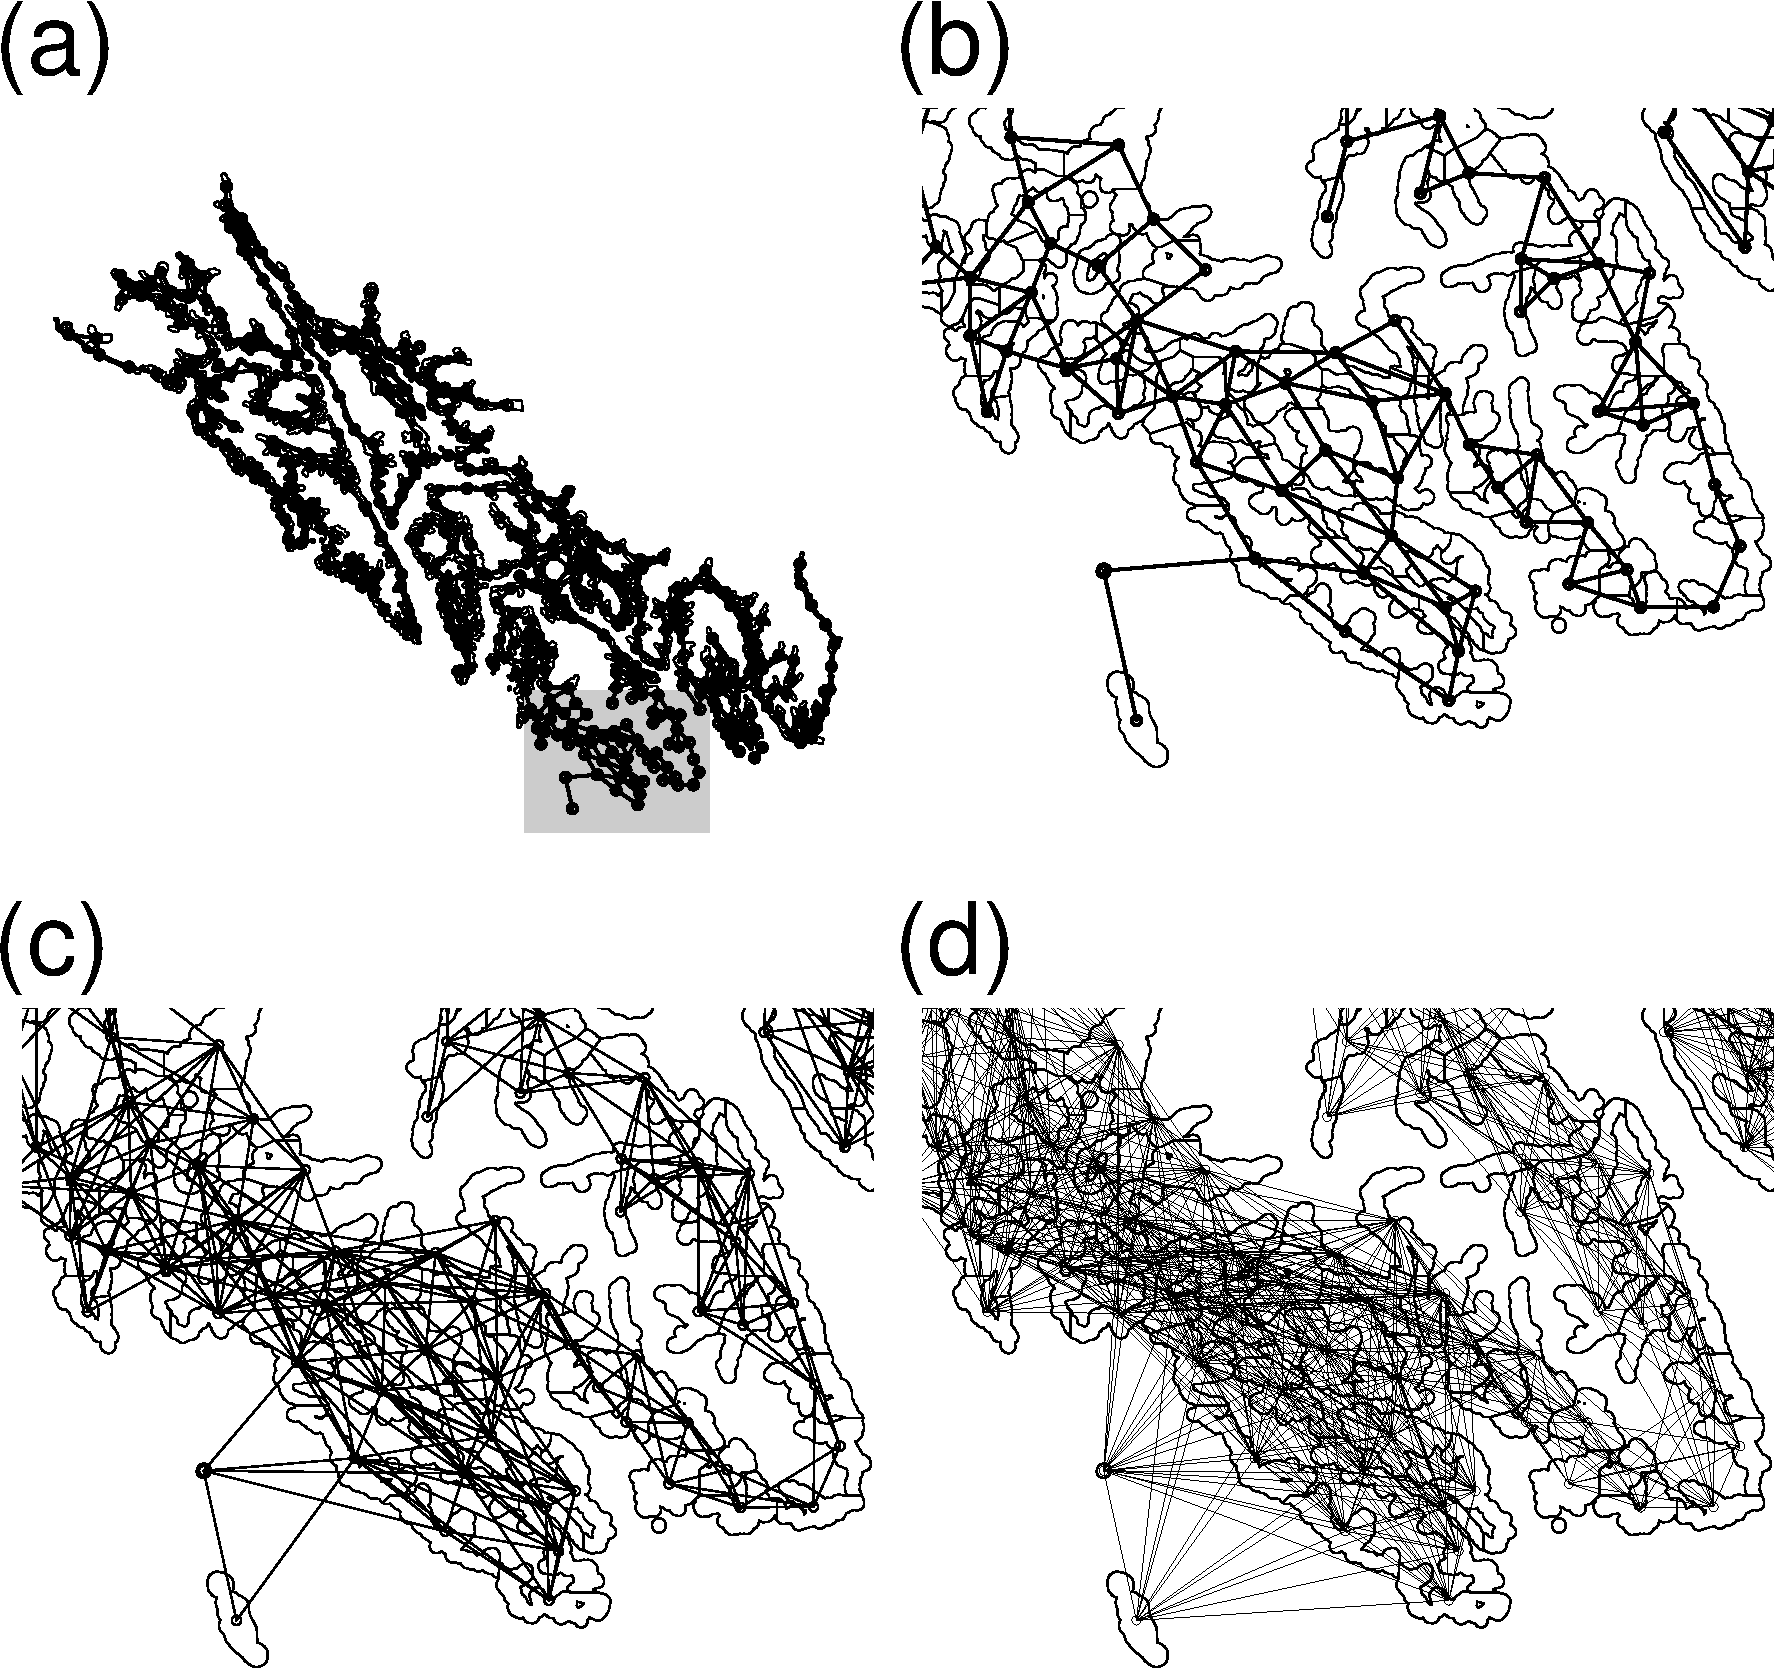
\includegraphics[width=\linewidth]{figure/Fig-Neighbors.png}
  \end{center}
  \caption{First, second, and fourth-order neighbor definitions for the survey polygons. (a) First-order neighbors for all polygons.  The grey rectangle is the area for a closer view in the following subfigures: (b) first-order neighbors; (c) second-order neighbors; and (d) fourth-order neighbors. \label{Fig-Neighbors}}     
\end{figure}


%------------------------------------------------------------------------------
%                   Fig-ModelsM2LL
%------------------------------------------------------------------------------


\begin{figure}[H]
  \begin{center}
  \includegraphics[width=\linewidth]{figure/Fig-ModelsM2LL-crop.pdf}
  \end{center}
  \caption{Two times the log-likehood for the optimized (maximized) fit for the models given in Table~\ref{Tab:Models}. Model mU had a much lower value (350.2) and is not shown. Starting with model XU, the dashed grey lines show increments of 2, which helps evaluate the relative importance of models by either an AIC or a likelihood-ratio test criteria. \label{Fig-ModelsM2LL}}     
\end{figure}

%------------------------------------------------------------------------------
%                   Fig-rhoProfile
%------------------------------------------------------------------------------


\begin{figure}[H]
  \begin{center}
  \includegraphics[width=.9\linewidth]{figure/Fig-rhoProfile-crop.pdf}
  \end{center}
  \caption{The different lines show 2$*$log-likelihood profiles of $\rho$ for three different models, listed in the legend.  If the model is followed by -MLE, then the maximum of the profile provides the maximum likelihood estimate, and the 2$*$log-likelihood is given by the left y-axis, while if it is followed by MCMC, then it is the posterior distribution from a Bayesian model with a uniform prior on $\rho$, and the density is given by the right y-axis.  The horizontal dotted line is the maximum value for XC4R minus 3.841, the 0.05 $\alpha$-level value of a $\chi$-squared distribution on one degree of freedom. \label{Fig-rhoProfile}}     
\end{figure}

%------------------------------------------------------------------------------
%                   Fig-thetaProfiles
%------------------------------------------------------------------------------


\begin{figure}[H]
  \begin{center}
  \includegraphics[width=\linewidth]{figure/Fig-thetaProfiles-crop.pdf}
  \end{center}
  \caption{A) The solid line is the 2*Log-likelihood profile of $\theta_2$ for model XC4RD. B) The solid line is the 2*Log-likelihood profile of $\theta_1$ for model XC4RDS.  For each figure, the horizontal dashed line is the maximum value for the model minus 3.841, the 0.05 $\alpha$-level value of a $\chi$-squared distribution on one degree of freedom. \label{Fig-thetaProfiles}}     
\end{figure}


%------------------------------------------------------------------------------
%                   Fig-PredSmoo
%------------------------------------------------------------------------------


\begin{figure}[H]
  \begin{center}
  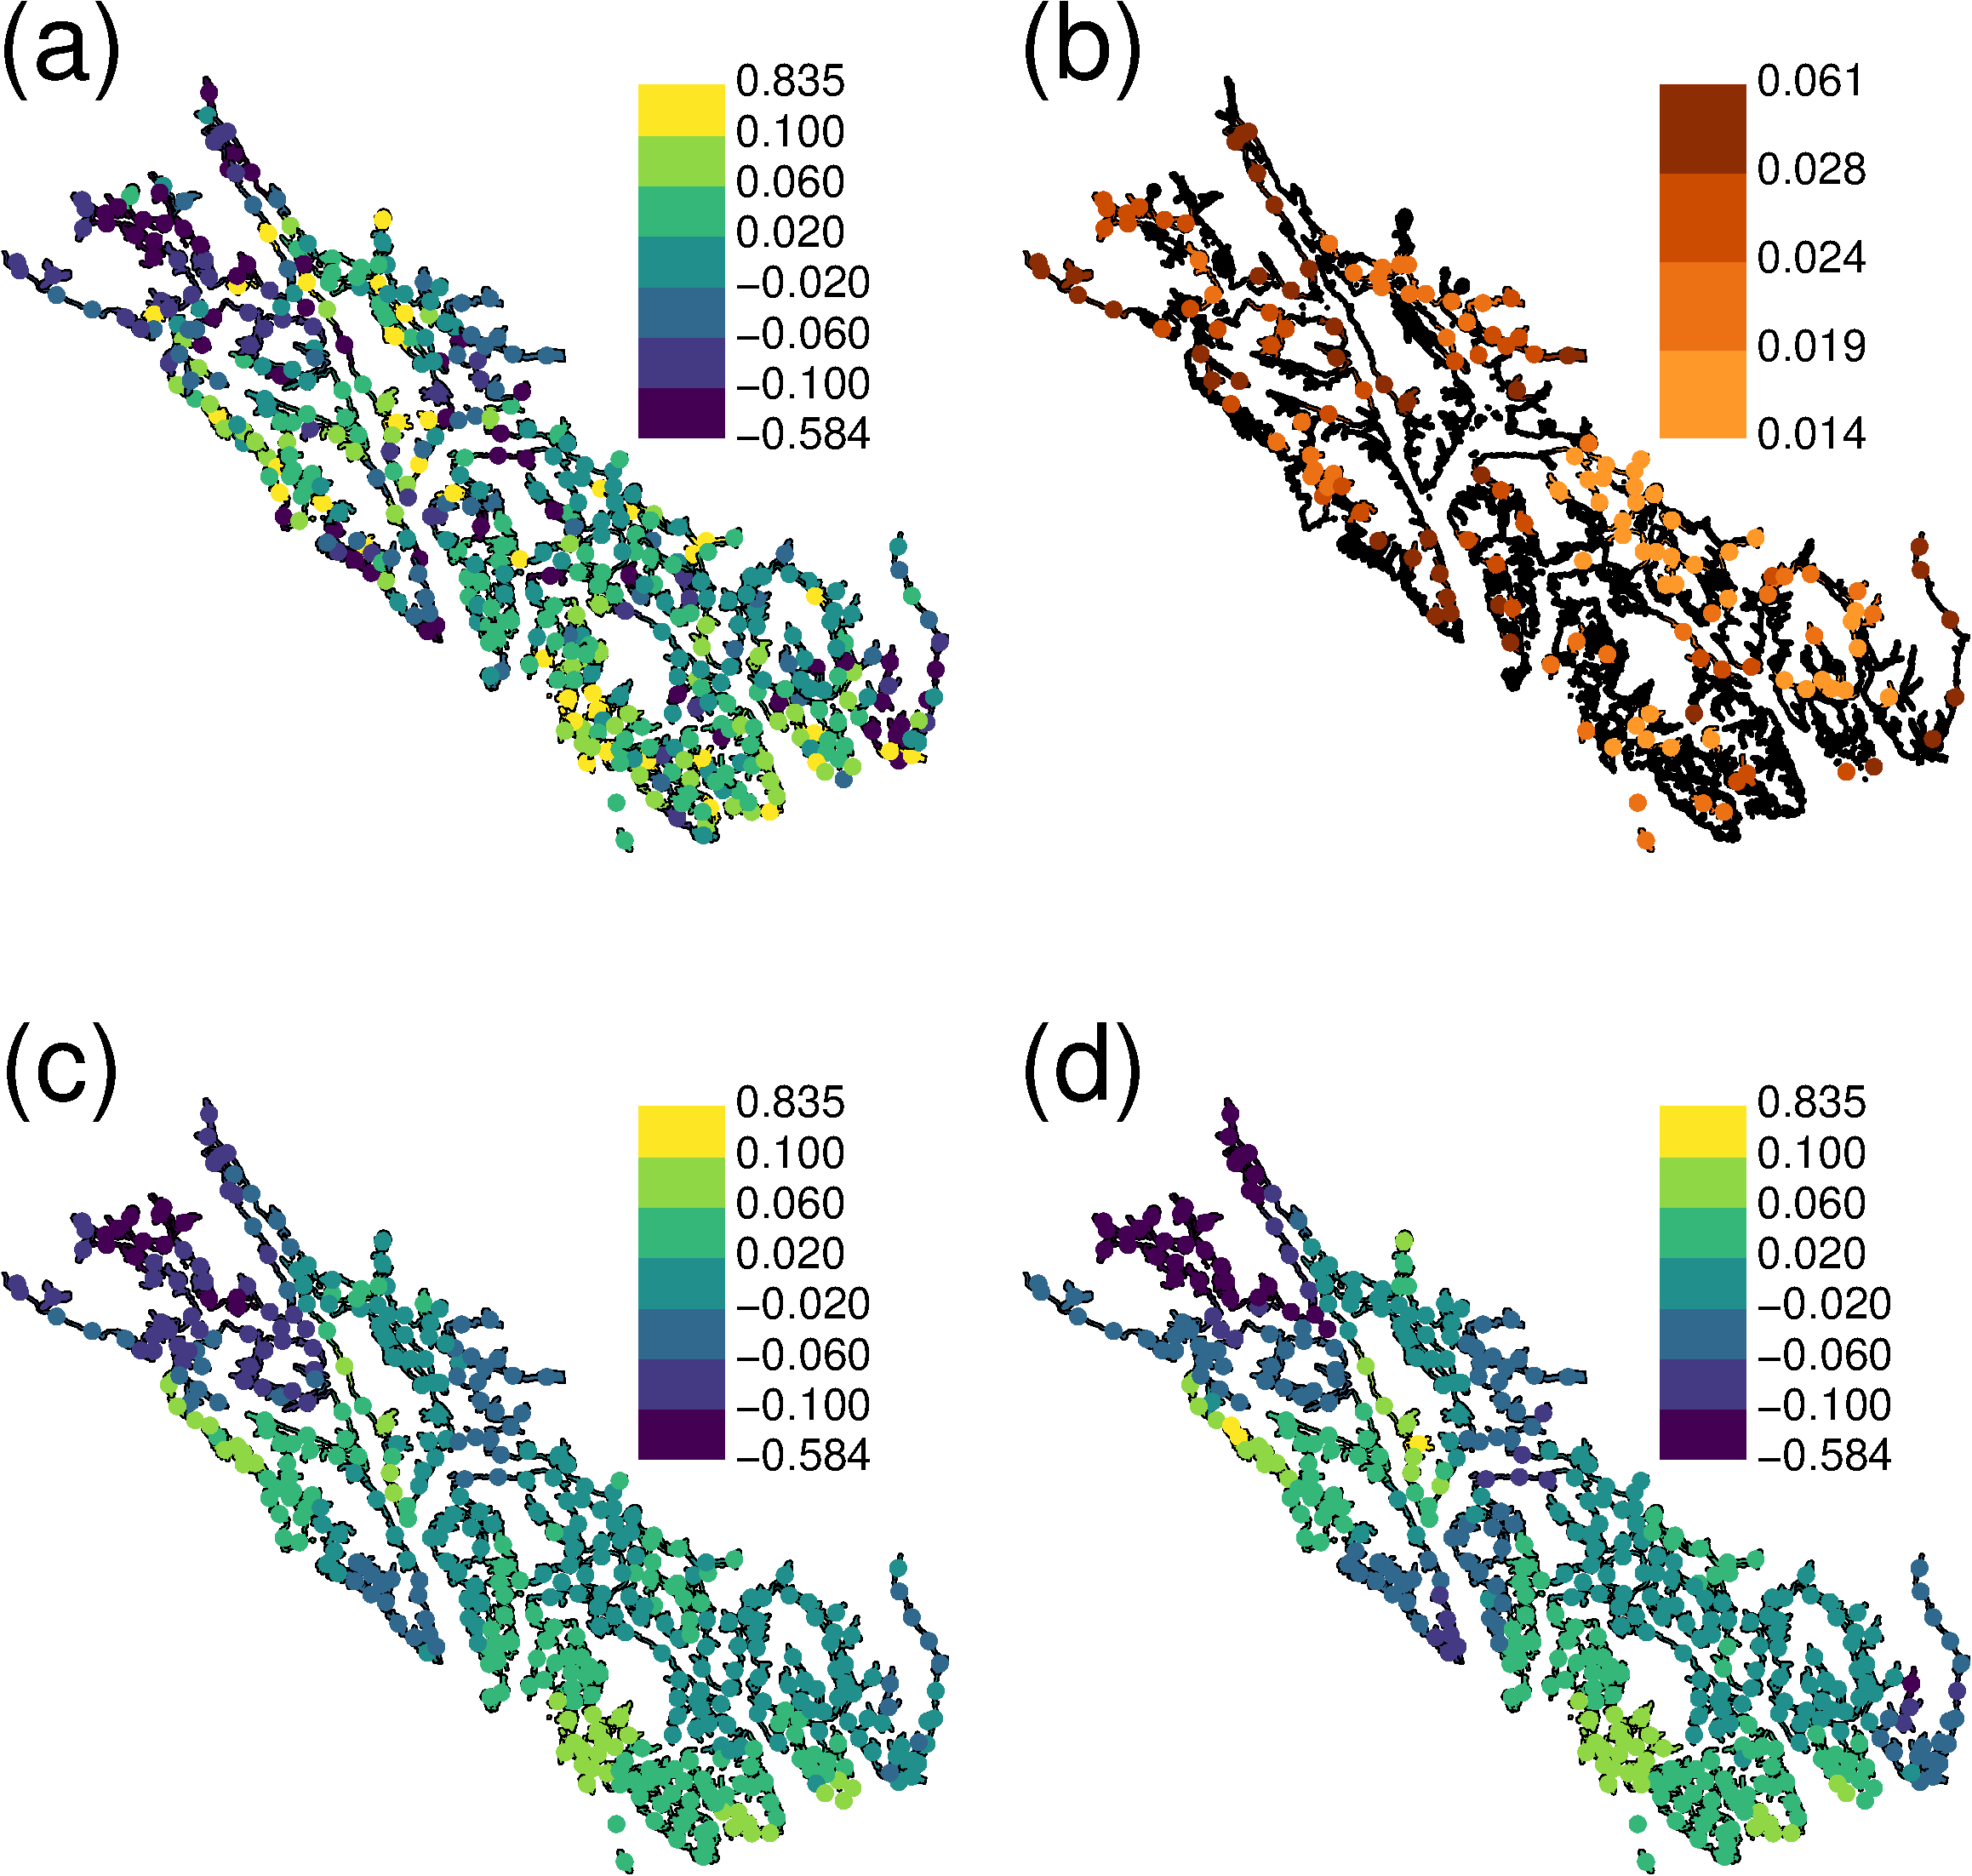
\includegraphics[width=\linewidth]{figure/Fig-PredSmoo.png}
  \end{center}
  \caption{Predictions and smoothing for the harbor-seal stock-trend data. (a) Predictions, using universal kriging from the XC4R model, at unsampled locations have been added to the raw observed data from sampled locations. (b) Prediction standard errors for unsampled locations using universal kriging from XC4R. (c) Smoothing over all locations using conditional expectation based on the XC4R model.  (d) Smoothing over all locations by using posterior predictions (mean of posterior distributions) using the XI4RU model in a Bayesian hierarchical model.  \label{Fig-PredSmoo}}     
\end{figure}


%------------------------------------------------------------------------------
%                   Fig-MargVar
%------------------------------------------------------------------------------


\begin{figure}[H]
  \begin{center}
  \includegraphics[width=.7\linewidth]{figure/Fig-MargVar.png}
  \end{center}
  \caption{Nonstationarity illustrated for XC4 model, and the same model using row-standardization, XC4R.  A) Marginal variances of the multivariate covariance matrix (diagonal elements of $\bSigma$) as a function of the numbers of neighbors, where circles indicate XC4R and squares indicate XC4.  Each symbol is partially transparent. B) All pairwise correlations as a function of the neighborhood order between sites. On the left of each neighbor order is XC4R, and on the right is XC4.  The larger circle is the average value. C) and D) Boxplots of pairwise correlation as a function of distance between polygon centroids, binned into classes, for models XC4R and XC4, respectively. \label{Fig-MargVar}}     
\end{figure}




%%%%%%%%%%%%%%%%%%%%%%%%%%%%%%%%%%%%%%%%%%%%%%%%%%%%%%%%%%%%%%%%%%%%%%%%%%%%%%%%%%
%%%%%%%%%%%%%%%%%%%%%%%%%%%%%%%%%%%%%%%%%%%%%%%%%%%%%%%%%%%%%%%%%%%%%%%%%%%%%%%%%%
%              APPENDIX
%%%%%%%%%%%%%%%%%%%%%%%%%%%%%%%%%%%%%%%%%%%%%%%%%%%%%%%%%%%%%%%%%%%%%%%%%%%%%%%%%%
%%%%%%%%%%%%%%%%%%%%%%%%%%%%%%%%%%%%%%%%%%%%%%%%%%%%%%%%%%%%%%%%%%%%%%%%%%%%%%%%%%

%------------------------------------------------------------------------------
%          Appendix A: Misconceptions and Errors in the Literature
%------------------------------------------------------------------------------

\clearpage
\setcounter{equation}{0}
\renewcommand{\theequation}{A.\arabic{equation}}
\setcounter{figure}{0}
\renewcommand{\thefigure}{A.\arabic{figure}}
\section{APPENDIX A: Misconceptions and Errors in the Literature}

The fact that CAR and SAR models are developed for the precision matrix, in contrast to geostatistical models being developed for the covariance matrix, has caused some confusion in the ecological literature.  For example, in comparing geostatistical models to SAR models, \citet{Begu:Puey:comp:2009} stated ``Semivariogram models account for spatial autocorrelation \emph{at all possible distance lags}, and thus they do not require \emph{a priori} specification of the window size and the covariance structure,'' (emphasis by the original authors).  CAR and SAR models also account for spatial autocorrelation at all possible lags, as seen in Fig.~\ref{Fig-MargVar}c,d.  In a temporal analogy, the autoregressive AR1 time series models also account for autocorrelation at all possible lags, where the conditional specification $Z_{i+1} = \phi Z_i + \nu_i$, with $\nu_i$ an independent random shock and $|\phi| < 1$, implies that $\corr(Z_{i},Z_{i+t}) = \phi^t$ for all $t$.  In fact, if we restrict $0 < \phi < 1$, then this can be reparameterized as $\corr(Z_{i},Z_{i+t}) = \exp(-t(-\log(\phi)))$, which is an exponential geostatistical model with range parameter $-\log(\phi)$.  While there are interesting results in \citet{Begu:Puey:comp:2009}, a restriction on the range of autocorrelation is not a reason that CAR/SAR models might perform poorly against a geostatistical model.  The important concept is that the autoregressive specification is local in the precision matrix and not in the covariance matrix.

CAR models are often incorrectly characterized.  For example, \citet{Keit:Bjor:Dixo:Citr:acco:2002} characterized CAR models as: $\bY = \bX\bbeta + \rho\bC(\bY - \bX\bbeta) + \bvarepsilon$, with a stated covariance matrix of $\sigma^2(\bI - \rho\bC)\upi$, where $\bC$ is symmetric. Their actual implementation may have been correct, and there are excellent and important results in \citet{Keit:Bjor:Dixo:Citr:acco:2002}; however, the construction they used leads to a SAR covariance matrix of $\sigma^2(\bI - \rho\bC)\upi(\bI - \rho\bC)\upi$ if $\var(\bvarepsilon) = \sigma^2\bI$ and $\bC$ is symmetric. Even to characterize a CAR model as $\sigma^2(\bI - \rho\bC)\upi$ with symmetric $\bC$ is overly restrictive, as we have demonstrated that an asymmetric $\bC$ with the proper $\bM$ will still satisfy Eq. \ref{eq:CarSymmetry}, or alternatively that $\bSigma\upi = (\bM\upi - \bC)/\sigma^2$, where $\bC$ is symmetric but $\bM\upi$ is not necessarily constant on the diagonals. In fact, constraining a CAR model to $\sigma^2(\bI - \rho\bC)\upi$ does not allow for row-standardized models.  These mistakes are perpetuated in \citet{Dorm:etal:meth:2007}, and we have seen similar errors in describing CAR models as SAR models in other literature, presentations, and help sites on the internet. 

\citet{Dorm:etal:meth:2007} also claimed that any SAR model is a CAR model, which agrees with the literature \citep[e.g.,][p. 409]{Cres:stat:1993}, but then they show an incorrect proof (it is also incorrect in \citet[][p. 89]{Hain:spat:1990}, and likely beginning there), because they do not consider that $\bC$ for a CAR model must have zeros along the diagonal.  In fact, we demonstrate in Appendix B that, despite statistical and ecological literature to the contrary, CAR models and SAR models can be written equivalently, and we provide details.

%------------------------------------------------------------------------------
%          Appendix B: Equivalence of CAR and SAR Models
%------------------------------------------------------------------------------

\clearpage
\setcounter{equation}{0}
\renewcommand{\theequation}{B.\arabic{equation}}
\setcounter{figure}{0}
\renewcommand{\thefigure}{B.\arabic{figure}}
\section{APPENDIX B: Equivalence of CAR and SAR Models}

In what follows, for matrices denoted with bold capital letters, let their $i$th column and $j$ row be denoted with small case letters with subscripts $i,j$; for example, the $i,j$th element of $\bC$ is $c_{ij}$.  Assume $\bM$ and $\bLambda$ are diagonal matrices. To establish when CAR models can be written as SAR, and vice versa, we need the following equality,
\begin{equation} \label{eq:CAReqSAR}
(\bI-\bC)\upi\bM = (\bI - \bB)\upi\bLambda(\bI - \bB\upp)\upi,
\end{equation}
satisfying, for the CAR covariance matrix on the left-hand side,
\newcounter{saveenum}
\begin{enumerate}[1)]
  \item $(\bI-\bC)\upi$ exists, 
	\item  $c_{ii} = 0, \, \forall \, i$, and
	\item $c_{ij}/m_{ii}=c_{ji}/m_{jj}, \; \forall \; i,j$;
	\setcounter{saveenum}{\value{enumi}}
\end{enumerate}
and for the SAR covariance matrix on the right-hand side,
\begin{enumerate}[1)]
	\setcounter{enumi}{\value{saveenum}}
	\item $(\bI-\bB)\upi$ exists, and 
	\item $b_{ii} = 0, \; \forall \; i$.  
\end{enumerate}
Notice that we write the SAR covariance matrix as $(\bI - \bB)\upi\bLambda(\bI - \bB\upp)\upi$, where $\bLambda$ is a diagonal matrix, in Eq. \ref{eq:CAReqSAR}, following \citet[p. 409]{Cres:stat:1993}, which is a little more general than the SAR covariance matrix given in Eq. \ref{eq:SARcov}.  Ultimately, this demonstration relies on establishing that any zero-mean Gaussian distribution on a finite set of points, $\bZ \sim N(\bzero,\bSigma)$, can be written as either the left-hand side, or the right-hand side of Eq. \ref{eq:CAReqSAR}.  Note, we make use of the following results. If $\bD$ is diagonal, and $\bQ$ has zero on the diagonals, then both $\bD\bQ$ and $\bQ\bD$ have zeros on the diagonal. If $\bA = \bB\bC$, and $\bA$ and $\bC$ have inverses, then $\bB$ has an inverse. 

First consider obtaining the left-hand side of Eq. \ref{eq:CAReqSAR}; this result is also given by \citet[p. 434]{Cres:stat:1993}. Write $\bSigma\upi = \bD - \bQ$, where $\bD$ is diagonal and $\bQ$ has zeros on the diagonal.  Then factor out $\bD$ so that $\bSigma\upi = \bD(\bI - \bD\upi\bQ)$, and now let $\bM = \bD\upi$ and $\bC = \bD\upi\bQ$, then $(\bI - \bC)\upi$ exists because $\bSigma\upi$ and $\bD\upi$ exist, $\bC$ will have zeros on the diagonals, and condition 3) is satisfied by construction (because it is the requirement for symmetry).  Thus, $\bSigma\upi$ can be expressed as $\bM\upi(\bI - \bC)$ and $\bSigma = (\bI-\bC)\upi\bM$ satisfying conditions 1) to 3).

Next, consider the right-hand side of Eq. \ref{eq:CAReqSAR}. Write $\bSigma\upi = \bL\bL\upp$, and suppose that $\bL$ has an inverse. Note that $\bL$ is \emph{not} unique.  A Cholesky decomposition satisfies this, where $\bL$ is lower triangular, or a singular value decomposition could be used, where $\bSigma = \bV\bE\bV\upp$ with $\bV$ containing orthonormal eigenvectors and $\bE$ containing eigenvalues. Then $\bL = \bV\bE^{-1/2}\bV\upp$. In any case, let  $\bL\bL\upp = (\bG - \bP)(\bG\upp - \bP\upp)$, where $\bG$ is diagonal and $\bP$ has zero diagonals. Then factor out $\bG$ to obtain $\bL\bL\upp = (\bI - \bP\bG\upi)\bG\bG(\bI - \bG\upi\bP\upp)$, and now let $\bLambda\upi = \bG\bG$ and $\bB\upp = \bP\bG\upi$.  Notice that $(\bP\bG\upi)\upp = \bG\upi\bP\upp$ because $\bG\upi$ is diagonal. Thus, $\bSigma\upi$ can be expressed as $(\bI - \bB\upp)\bLambda\upi(\bI - \bB)$ and $\bSigma = (\bI - \bB)\upi\bLambda(\bI - \bB\upp)\upi$. Moreover, $(\bI - \bB)\upi$ exists because $\bL\upi$ and $\bG\upi$ exist and $\bB$ will have zeros on the diagonals, satisfying conditions 4) and 5).  Note that in order to write it as $(\bI - \bB)\upi(\bI - \bB\upp)\upi$, we would need to find $\bL$ with ones on the diagonal so that $\bG = \bI$.

Hence, we have demonstrated that any zero-mean Gaussian distribution on a finite set of points, $\bZ \sim \textrm{N}(\bzero,\bSigma)$ can be written as either the left-hand side, or the right-hand side of Eq. \ref{eq:CAReqSAR}, with the important difference that a CAR model is uniquely determined from $\bSigma$ but a SAR model is not so uniquely determined.  That a CAR is unique is easy to see from the algebra used to derive it.  To see more fully why a SAR model is not uniquely determined, let $\bA$ be a matrix with orthonormal columns, and notice that $\bSigma\upi = \bL\bL\upp = \bL(\bA\upp\bA)\bL\upp = (\bL\bA\upp)(\bA\bL\upp) = \bL_*\bL_*\upp$.  A SAR model can be developed as readily for $ \bL_*$ as for $\bL$.  In fact, if we think of $\bA$ as coordinate vectors, any rotation of the matrix $\bA$ will create yet another SAR model, so there are an infinite number of them.

With this appendix, we also wish to correct an error that has been perpetuating in the literature, beginning with \citet[p. 89]{Hain:spat:1990}, and we also found it in \citet{Scha:Gotw:stat:2005} and \citet{Dorm:etal:meth:2007}. The authors assume in Eq. \ref{eq:CAReqSAR} that $\bM = \bI$ and $\bLambda = \bI$, so that $\bC$ is symmetric.  That implies that $(\bI-\bC)\upi$ = $[(\bI - \bB)(\bI - \bB\upp)]\upi$ =$(\bI - \bB - \bB\upp + \bB\bB\upp)\upi$, and the claim is that this shows how any SAR can be easily made into a CAR by setting $\bC = \bB + \bB\upp - \bB\bB\upp$. However, while $\bC = \bB + \bB\upp - \bB\bB\upp$ is sufficient for equality, it is not necessary, and it lacks a critical component; that $\bB + \bB\upp - \bB\bB\upp$ must have zeros on the diagonal for $\bC$ to be a CAR model. The proper way to proceed was outlined above, by letting $\bC = \bD\upi\bQ$ in the equality 
\[
(\bI - \bD\upi\bQ)\upi\bD\upi = (\bI - \bB - \bB\upp + \bB\bB\upp)\upi,
\]
where the left-hand side is uniquely determined from the right-hand size, and $\bC$ satisfies the requirement for a CAR model.  As we demonstrated in the previous paragraph, it is not possible to go uniquely from the left-hand side to the right-hand side without additional constraints.

%------------------------------------------------------------------------------
%Appendix C: Maximum Likelihood Estimation for CAR/SAR Models with Missing Data
%------------------------------------------------------------------------------

\clearpage
\setcounter{equation}{0}
\renewcommand{\theequation}{C.\arabic{equation}}
\setcounter{figure}{0}
\renewcommand{\thefigure}{C.\arabic{figure}}
\section{APPENDIX C: Maximum Likelihood Estimation for CAR/SAR Models with Missing Data}

We begin by finding analytical solutions when we can, and then substituting them into the likelihood to reduce the number of parameters as much as possible for the full covariance matrix.  Assume a linear model,
\[
  \by = \bX\bbeta + \bvarepsilon,
\]
where $\by$ is a vector of response variables, $\bX$ is a design matrix of full rank, $\bbeta$ is a vector of parameters, and the zero-mean random errors have a multivariate normal distribution, $\bvarepsilon \sim \textrm{N}(\bzero,\bSigma)$, where $\bSigma$ is a patterned covariance matrix; i.e., it has non-zero off-diagonal elements.  Suppose that $\bSigma$ has parameters $\{\theta,\brho\}$ and can be written as $\bSigma = \theta\bV_{\brho}$, where $\theta$ is an overall variance parameter and $\brho$ are parameters that structure $\bV_{\brho}$ as a non-diagonal matrix, and we show the dependency as a subscript. Note that $\bSigma\upi = \bV\upi_{\brho}/\theta$. Recall that the maximum likelihood estimate of $\bbeta$ for any $\{\theta,\brho\}$ is $\hat{\bbeta} = (\bX\upp\bV\upi_{\brho}\bX)\upi\bX\bV\upi_{\brho}\by$. By substituting $\hat{\bbeta}$ into the normal likelihood equations, $-2$ times the loglikelihood for a normal distribution is
\[
  \cL(\theta,\brho|\by) = (\by - \bX\hat{\bbeta})\upp\bSigma\upi(\by - \bX\hat{\bbeta}) + \log(|\bSigma|) + n\log(2\pi),
\]
where $n$ is the length of $\by$, but this can be written as,
\begin{equation}\label{eq:MVNloglike}
\cL(\theta,\brho|\by) = \br_{\brho}\upp\bV\upi_{\brho}\br_{\brho}/\theta + n\log(\theta) + \log(|\bV|) + n\log(2\pi)
\end{equation}
where $\br_{\brho} = (\by - \bX\hat{\bbeta})$ (notice that $\hat{\bbeta}$ is a function of $\brho$, so we show that dependency for $\br$ as well).  Conditioning on $\brho$ yields 
\[
\cL(\theta|\brho,\by) = \br_{\brho}\upp\bV\upi_{\brho}\br_{\brho}/\theta + n\log(\theta)+ \textrm{terms not containing } \theta
\]
and minimizing for $\theta$ involves setting
\[
\frac{\partial \cL(\theta|\brho,\by)}{\partial \theta} = -\br\upp_{\brho}\bV\upi_{\brho}\br_{\brho}/\theta^2 + n/\theta
\]
equal to zero, yielding the maximum likelihood estimate
\begin{equation}\label{eq:MLEtheta}
 \hat{\theta} = \br\upp_{\brho}\bV\upi_{\brho}\br_{\brho}/n.
\end{equation}
Substituting Eq. \ref{eq:MLEtheta} back into Eq. \ref{eq:MVNloglike} yields the -2*loglikelihood as a function of $\brho$ only,
\begin{equation}\label{eq:MVNrhoOnly}
\cL(\brho|\by) = n\log(\br\upp_{\brho}\bV\upi_{\brho}\br_{\brho}) + \log(|\bV_{\brho}|) + n(\log(2\pi) + 1 - \log(n)). 
\end{equation}
Equation Eq. \ref{eq:MVNrhoOnly} can be minimized numerically to yield the MLE $\hat{\brho}$, and then $\hat{\theta} = \br\upp_{\hat{\brho}}\bV\upi_{\hat{\brho}}\br_{\hat{\brho}}/n$, and  $\hat{\bbeta} = (\bX\upp\bV\upi_{\hat{\brho}}\bX)\upi\bX\bV\upi_{\hat{\brho}}\by$.

We developed the inverse covariance matrix $\bSigma_A\upi = \textrm{diag}(\bW\bone) - \rho\bW)$, and here we use $\bSigma_A$ to denote it is for \emph{all} locations, those with observed data as well as those without. Without missing data, Eq. \ref{eq:MVNrhoOnly} can be evaluated quickly by factoring out an overall variance parameter from $\bSigma_A\upi$ and using sparse matrix methods to quickly and efficiently evaluate $|\bV_{\brho}|$ by recalling that $|\bV_{\brho}|$ = $1/|\bV\upi_{\brho}|$.  However, when there are missing data, there is no guarantee that $\bV_{\brho}$ will be sparse.  The obvious and direct approach is to first obtain $\bSigma_A = (\bSigma_A\upi)\upi$, and then obtain $\bV_{\brho} = \bSigma[\bi,\bi]$, where $\bi$ is a vector of indicators that subsets the rows and columns of $\bSigma$ to only those for sampled locations.  Then, a third step is a second inverse to find $\bV_{\brho}\upi$.  However, this is computationally expensive.  A faster way uses results from partitioned matrices and Schur complements.  In general, let the square matrix $\bSigma$ with dimensions $(m + n) \times (n + m)$ be partitioned into block submatrices,
\[
  \underset{(m+n) \times (m+n)}{\bSigma} = \left[
    \begin{array}{cc}
	    \underset{m \times m}{\bA} & \underset{m \times n}{\bB} \\
	    \underset{n \times m}{\bC} & \underset{n \times n}{\bD}
    \end{array}
  \right]
\]
with dimensions given below each matrix. Assume $\bA$ and $\bD$ are nonsingular.  Then define the matrix function $\bS(\bSigma,\bA) = \bD - \bC\bA\upi\bB$ as the Schur complement of $\bSigma$ with respect to $\bA$.  Likewise, there is a Schur complement with respect to $\bD$ by reversing the roles of $\bA$ and $\bD$.  Using Schur complements, it is well-known \citep[e.g,][p. 97]{Harv:matr:1997} that an inverse for a partitioned matrix $\bSigma$ is,
\[
  \bSigma\upi = \left[
    \begin{array}{cc}
      \bA\upi + \bA\upi\bB\bS(\bSigma,\bA)\upi\bC\bA\upi & -\bA\upi\bB\bS(\bSigma,\bA)\upi \\
      -\bS(\bSigma,\bA)\upi\bC\bA\upi & \bS(\bSigma,\bA)\upi
    \end{array}
  \right]
\]
Then, note that $\bA\upi = \bS(\bSigma\upi, \bS(\bSigma,\bA)\upi)$; that is, if we already have $\bSigma\upi$, then $\bA\upi$ is the Schur complement of $\bSigma\upi$ with respect to the rows and columns that correspond to $\bD$.  Additionally, the largest matrix that we have to invert is $[\bS(\bSigma,\bA)\upi]\upi$, which is $n \times $n, which has dimension less than $\bSigma$, and only one inverse is required. So, if we let $\bA$ correspond to the rows and columns of the observed locations, and $\bD$ correspond to the rows and columns of the missing data, then this provides a quick and efficient way to obtain $\bV_{\brho}\upi$ from $\bSigma_A\upi$, and the largest inverse required is $n \times n$, the number of missing data.

%------------------------------------------------------------------------------
%                 Appendix D: Prediction and Smoothing
%------------------------------------------------------------------------------

\clearpage
\setcounter{equation}{0}
\renewcommand{\theequation}{D.\arabic{equation}}
\setcounter{figure}{0}
\renewcommand{\thefigure}{D.\arabic{figure}}
\section{APPENDIX D: Prediction and Smoothing}

Here, we provide the formulas used in creating Fig.~\ref{Fig-PredSmoo}.  For universal kriging, the formulas can be found in \citet[][p. 148]{Cres:Wikl:stat:2011},
\[
				\hat{y}_i = \bx_i\upp\hat{\bbeta} + \bc_i\bSigma\upi_{-i}(\by_{-i} - \bX\hat{\bbeta})
\]
where $\hat{y}_i$ is the prediction for the $i$th node, $\bx_i$ is a vector containing the covariate values for the $i$th node, $\bX$ is the design matrix for the covariates (fixed effects), $\bc_i$ is a vector containing the fitted covariance between the $i$th site and all \emph{other} sites with observed data, $\bSigma$ is the fitted covariance matrix among all observed data, $\by$ is a vector of observed values for the response variable, and $\hat{\bbeta} = \bX\upp(\bX\upp\bSigma\upi\bX)\upi\bX\upp\bSigma\upi\by$ is the generalized least squares estimate of $\bbeta$.  The covariance values contained in $\bc_i$ and $\bSigma$ were obtained using maximum likelihood estimate for the parameters as detailed in Appendix C.  We include the $-i$ subscript on $\bSigma\upi_{-i}$ and $\by_{-i}$ to indicate that, when smoothing, we predict at the $i$th node by removing that datum from $\by$, and by removing its corresponding rows and columns in $\bSigma$.  If the value is missing, then prediction proceeds using all observed values.  Hence, Fig.~\ref{Fig-PredSmoo}a contains the observed values plus the predicted values at nodes with missing values, while Fig.~\ref{Fig-PredSmoo}c contains predicted values at all nodes, where any observed value at a node was removed and predicted with the rest of the observed values.  The prediction standard errors are given by,
\[
	\hat{\textrm{se}}(\hat{y}_i) = \sqrt{\bc_i\upp\bSigma\upi_{-i}\bc_i + 
	  \bd_i\upp(\bX_{-i}\upp\bSigma\upi_{-i}\bX_{-i})\upi \bd_i}
\]
where $\bd_i = \bx_i\upp - \bX_{-i}\upp\bSigma\upi_{-i}\bc_i$.

For the IAR model smoothing in Fig.~\ref{Fig-PredSmoo}d, we used the WinBUGS \citep{Lunn:Thom:Best:Spie:winb:2000} software, final version 1.4.3.  The model code is very compact and given below:
\begin{Verbatim}[baselinestretch=0.75]
model
  {
    for(i in 1:N) {
      trend[i] ~ dnorm(mu[i],prec)
      mu[i] <- beta0 + beta[stockid[i]] + b[i]
	  }
    b[1:N] ~ car.normal(adj[], weights[], num[], tau)
    beta0 ~ dnorm(0,.001)
    beta[1] ~ dnorm(0,.001)
    beta[2] ~ dnorm(0,.001)
    beta[3] ~ dnorm(0,.001)
    beta[4] <- 0
    beta[5] ~ dnorm(0,.001)
    prec ~ dgamma(0.001,0.001)
    sigmaEps <- sqrt(1/prec)
    tau  ~ dgamma(0.5, 0.0005) 
    sigmaZ <- sqrt(1 / tau)		
  }
\end{Verbatim}
The means of the MCMC samples from the posterior distributions of \texttt{mu[i]} were used for the IAR smoothing for the $i$th location in Fig.~\ref{Fig-PredSmoo}d.

%%%%%%%%%%%%%%%%%%%%%%%%%%%%%%%%%%%%%%%%%%%%%%%%%%%%%%%%%%%%%%%%%%%%%%%%%%%%%%%%%%
%%%%%%%%%%%%%%%%%%%%%%%%%%%%%%%%%%%%%%%%%%%%%%%%%%%%%%%%%%%%%%%%%%%%%%%%%%%%%%%%%%
%%%%%%%%%%%            %%%%%%%    %%%%%%%%  %%%%%%%       %%%%%%%%%%%%%%%%%%%%%%%%
%%%%%%%%%%%  %%%%%%%%%%%%%%%%%  %  %%%%%%%  %%%%%%%  %%%%  %%%%%%%%%%%%%%%%%%%%%%%
%%%%%%%%%%%  %%%%%%%%%%%%%%%%%  %%  %%%%%%  %%%%%%%  %%%%%%  %%%%%%%%%%%%%%%%%%%%%
%%%%%%%%%%%  %%%%%%%%%%%%%%%%%  %%%  %%%%%  %%%%%%%  %%%%%%%   %%%%%%%%%%%%%%%%%%%
%%%%%%%%%%%            %%%%%%%  %%%%  %%%%  %%%%%%%  %%%%%%%%  %%%%%%%%%%%%%%%%%%%
%%%%%%%%%%%  %%%%%%%%%%%%%%%%%  %%%%%  %%%  %%%%%%%  %%%%%%%   %%%%%%%%%%%%%%%%%%%
%%%%%%%%%%%  %%%%%%%%%%%%%%%%%  %%%%%%  %%  %%%%%%%  %%%%%%  %%%%%%%%%%%%%%%%%%%%%
%%%%%%%%%%%  %%%%%%%%%%%%%%%%%  %%%%%%%  %  %%%%%%%  %%%%  %%%%%%%%%%%%%%%%%%%%%%%
%%%%%%%%%%%            %%%%%%%  %%%%%%%%    %%%%%%%       %%%%%%%%%%%%%%%%%%%%%%%%
%%%%%%%%%%%%%%%%%%%%%%%%%%%%%%%%%%%%%%%%%%%%%%%%%%%%%%%%%%%%%%%%%%%%%%%%%%%%%%%%%%
%%%%%%%%%%%%%%%%%%%%%%%%%%%%%%%%%%%%%%%%%%%%%%%%%%%%%%%%%%%%%%%%%%%%%%%%%%%%%%%%%%

\end{flushleft}
\end{spacing}
\end{document}


